% !TeX root = main.tex
%--------------------------------------------------------%


%--------------------------------------------------------%
%	This is the main .tex file, which controls and combines
%	the other sections.
%	See the "sections" folder to edit content
%--------------------------------------------------------%

% !TeX root = ../main.tex

%--------------------------------------------------------%
% DOCUMENT CLASS
%--------------------------------------------------------%
% Change "letterpaper" to "a4" if you use a4 paper size
\documentclass[letterpaper,12pt]{article}

%--------------------------------------------------------%
% VIETNAMESE
%--------------------------------------------------------%

% \usepackage[T2A,T5]{fontenc}
% \usepackage[utf8]{inputenc}
% \usepackage[english,vietnamese]{babel}

\DeclareUnicodeCharacter{223C}{+}

%--------------------------------------------------------%
% TITLE SECTION
%--------------------------------------------------------%

%Abstract
\usepackage{abstract} % Allows abstract customization
% Set the "Abstract" text to bold
\renewcommand{\abstractnamefont}{\normalfont\bfseries}
\renewenvironment{abstract}{\par\noindent\textbf{\abstractname:}\ \ignorespaces}
% Set the abstract itself to small italic text
\renewcommand{\abstracttextfont}{\normalfont\small\itshape}

%Title
\usepackage{titlesec} % Allows customization of titles
\titlelabel{\thetitle.\quad}

%Authors
\usepackage{authblk} % For multiple authors
% \usepackage{cite} % Incompatible with biblatex
%Date
\usepackage{datetime} % allows for including today's date
% These two lines creates a new date format ``Month day(th), year''
\newdateformat{usvardate}{
    \monthname[\THEMONTH] \ordinal{DAY}, \THEYEAR}

%--------------------------------------------------------%
% HEADERS & FOOTERS
%--------------------------------------------------------%

%Footnotes
\usepackage[bottom]{footmisc} % Makes footnotes stick to bottom of the page

%Endnotes
% Uncomment this line if using endnotes "\endnote{}"
% \usepackage{endnotes}

%Headers from page 2 on
\usepackage{fancyhdr}
\pagestyle{fancy}
\fancyheadoffset{0cm}
\setlength{\headheight}{15pt}
\usepackage{comment}

%--------------------------------------------------------%
% DRAFT WATERMARK
%--------------------------------------------------------%

% NOTE: Comment out these two lines to remove watermark
% \usepackage[firstpage]{draftwatermark} % adds draft watermark
% \SetWatermarkLightness{0.85}

%--------------------------------------------------------%
% MACROS
%--------------------------------------------------------%
% Define keywords macro command
\providecommand{\keywords}[1]{\textbf{\textit{Keywords---}} #1}

%% LianTze 7 Dec 2016:
%% Updated how the wordcount is implemented
\newcommand\wordcount{%
    \immediate\write18{texcount -utf8 -merge -sum -incbib -dir -sub=none -brief \jobname.tex | cut -d : -f 1 > 'count.txt'}%
    \input{count.txt}\ignorespaces words%
}

%--------------------------------------------------------%
% MATH SUPPORT
%--------------------------------------------------------%

% The amssymb package provides various useful mathematical symbols
\usepackage{amssymb}
% The amsthm package provides extended theorem environments
\usepackage{amsthm}
% The newtxmath package provides additional math symbol support
% in Times New Roman symbols, etc.
\usepackage{newtxmath}
\usepackage{mathtools}
\usepackage{blkarray, bigstrut}

%--------------------------------------------------------%
% FONTS
%--------------------------------------------------------%

\usepackage{microtype} % Slightly tweak font spacing for aesthetics
\usepackage[utf8]{inputenc}
\usepackage{newtxtext} % Makes default font Adobe Times New Roman

%--------------------------------------------------------%
% LINES
%--------------------------------------------------------%

% Spacing
\usepackage{setspace} % See \doublespacing command at the top of content.tex
% Numbering
\usepackage{lineno,xcolor} 	% See \linenumbers at the top of content.tex
% Lists
\usepackage{enumitem}
\setlist{nosep}
\setlist[itemize]{leftmargin=*}

%--------------------------------------------------------%
% MARGINS
%--------------------------------------------------------%

%NOTE: All spaces in this template are in inches, because it is
% formatted for letterpaper (8.5 x 11 inch) paper. If you use a4
% paper, choose different sizes in millimeters or centimeters.
\usepackage[top=1.5in, bottom=1.5in, left=1in, right=1in]{geometry}

%--------------------------------------------------------%
% COMMENTS
%--------------------------------------------------------%

\usepackage[colorinlistoftodos]{todonotes} % allows margin comments
% See examples in content.tex, and here for manual: 
% http://www.ctan.org/pkg/todonotes
\usepackage{soul} % allows for highlighting

%--------------------------------------------------------%
% ACRONYMS
%--------------------------------------------------------%

\usepackage[nohyperlinks,nolist]{acronym} % Managing acronyms
\usepackage{pifont} % For \ding symbols

%--------------------------------------------------------%
% GRAPHICS
%--------------------------------------------------------%

\usepackage{graphicx,caption} % More advanced figure inclusion
\graphicspath{{figures/}} % Set the default folder for images
\usepackage{float} % For specifying table/figure locations, i.e. [ht!]
\usepackage{subcaption}

% The printlen command allows the user to print the exact text width or height.
% This is useful, when trying to create graphics (outside of LaTeX, of course)
% with the optimal dimensions. See here for usage: http://www.ctan.org/pkg/printlen
\usepackage{printlen}

\usepackage[section]{placeins} % Used to ensure that figures do not go into the next section

% TikZ for the CALM-Row pipeline diagram
\usepackage{tikz}
\usetikzlibrary{arrows.meta,positioning,fit,backgrounds,calc}

%--------------------------------------------------------%
% TABLES
%--------------------------------------------------------%

\usepackage{adjustbox} 	%adjust table
\usepackage{ragged2e}	%su dung cho \justifying
\usepackage{bm} %in dam trong bang dung cho cong thuc

\usepackage{longtable} % For long tables that span multiple pages
\newcommand{\sym}[1]{\rlap{#1}}% For symbols like *** in tables
\usepackage{tabularx} % Allows advanced table features
\newcolumntype{L}[1]{>{\raggedright\arraybackslash}p{#1}}
\newcolumntype{C}[1]{>{\centering\arraybackslash}p{#1}}
\newcolumntype{R}[1]{>{\raggedleft\arraybackslash}p{#1}}
\usepackage{relsize} % Allows precise adjustment of font size,
%useful for fitting tables to page width
\usepackage{multirow}

%--------------------------------------------------------%
% REFERENCES
%--------------------------------------------------------%
% adding biography
\usepackage{wrapfig}
\usepackage{graphicx}  % For including images
\usepackage{subcaption}  % For subfigures
\usepackage{adjustbox}

\usepackage{hyperref} % For hyperlinks in the PDF

% NOTE: This document uses bibtex for references
% because both style files for Sociology Journals are
% only available in .bst format. You can change to
% biblatex if you prefer below.

% Many thanks to Sociology Professor, 
% ChangHwan Kim at the University of Kansas. 
% for providing these .bst files here: 
% http://people.ku.edu/~chkim

% BIBTEX
% Comment out this line if using biblatex
%\usepackage{chicago} % AJS and ASR styles rely on chicago

% BIBLATEX
% NOTE: Uncomment out these three lines to use biblatex
% Be sure to put the biblio.bib file in biblatex format'
\usepackage{csquotes}
\usepackage[style=numeric-comp,backend=biber,sorting=none]{biblatex}

\bibliography{refs}

 % See preamble.tex to edit the overall layout

% Header from Page Three on: Edit below for left and right headers
\lhead{}
\rhead{}

%--------------------------------------------------------%
%	BEGIN DOCUMENT
%--------------------------------------------------------%

\begin{document}



%TC:ignore   %% This region is ignored for the word count
% COVER PAGE

%--------------------------------------------------------%
%	COVER PAGE
%--------------------------------------------------------%

\begin{titlepage}

  \newcommand{\HRule}{\rule{\linewidth}{0.5mm}} % Defines a new command for the horizontal lines, change thickness here

  \center % Center everything on the page


  %	HEADING SECTION

  %\textsc{\LARGE University Name}\\[1.5cm] % Name of your university/college
  \textsc{\Large Manuscript Submission}\\[0.5cm] % Major heading such as course name
  % \textsc{\large XXX
  % }
  % \\[0.5cm] % Minor heading such as course title

  %	TITLE SECTION

  \vspace{1.5 cm}
  \HRule \\[0.4cm]
  { \huge \bfseries CALM-Row: Navigation-Native Crop-Row Guidance from the Calibrated Box-Distribution Uncertainty of a Stock Edge Detector} % Title of your document
  \HRule \\[1.5cm]

  %	AUTHOR SECTION

  %{\em\Large\textbf Authors:}\\
  %\vspace{.5 cm}
  %First \textsc{Author}\\
  %Department of XYZ,\\
  %The University of ABC\\
  %\vspace{.5 cm}
  %Second \textsc{Author}\\
  %Department of XYZ,\\
  %The University of ABC\\
  %\vspace{.5 cm}
  %Third \textsc{Author}\\
  %Department of ABC,\\
  %XYZ University\\
  Manh V. Hoang\textsuperscript{$\dagger$1}, Thang M. Pham\textsuperscript{1} and Nam Do\textsuperscript{1}
  \vspace{1cm}


  \textsuperscript{1}University of Engineering and Technology, Vietnam National University, Hanoi 10000, Vietnam \\

  \textsuperscript{$\dagger$}Correspondence should be sent to \href{mailto:manhhv87@vnu.edu.vn}{manhhv87@vnu.edu.vn} \\

  \vspace{1.5 cm}
  {\large Submitted: \today}\\[3cm] % Date, change the \today to a set date if you want to be precise

  \vfill % Fill the rest of the page with whitespace

\end{titlepage}

%-----------------------------------------------------------------

\newpage % Comment out to remove cover page
%TC:endignore

\thispagestyle{empty} % Removes header on page two. Only needed if there is a coverpage

% TITLE SECTION

% Comment out one of the two lines below to include or exclude authors in article title. You may want to exclude them in case of a double-blind peer review submission, since authors appear on the cover page, and reviewers should not see the authors' names in the manuscript draft.

%-----------------------------------------------------------
%	TITLE SECTION - with authors
%-----------------------------------------------------------

% Article title
\title{\vspace{-15mm}\fontsize{21pt}{10pt}\selectfont\textbf{Know-When-to-Trust Crop-Row Guidance: Conformal Heading Intervals and a Risk-Controlled Steering Policy on a Stock Edge Detector}}
%\thanks{Draft manuscript. Please do not cite without the authors' permission.}}}

% Today's date
	\date{Submitted: \usvardate\today}

\makeatletter
\renewcommand{\@maketitle}{
\newpage
 \null
 \vskip 2em%
 \begin{center}%
  {\LARGE \@title \par}%
 \end{center}%
 \par} \makeatother

%%--------------------------------------------------------%
%	TITLE SECTION with authors
%--------------------------------------------------------%

% Article title
  \title{\vspace{-15mm}\fontsize{21pt}{10pt}\selectfont\textbf{Know-When-to-Trust Crop-Row Guidance: Conformal Heading Intervals and a Risk-Controlled Steering Policy on a Stock Edge Detector}}
  %\thanks{Draft manuscript. Please do not cite without the authors' permission.}}}

% Authors and Affiliations
  \author[1,*]{\large Hanh Bui Thi}
  \author[2]{\large Hoang Van Manh}
  \author[2]{\large Pham Manh Thang}
  \affil[1]{\normalsize Faculty of Fundamental Science, Phenikaa University, Yen Nghia, Ha-Dong district, Hanoi 10000, Vietnam}
  \affil[2]{\normalsize Faculty of Engineering Mechanics and Automation, University of Engineering and Technology, Vietnam National University, Hanoi 10000, Vietnam}
  \renewcommand\Authands{ and }

% Today's date
	\date{Submitted: \usvardate\today}


\maketitle % Insert title

% NOTE: Comment out the lines below to remove line numbers
% Running line numbers:
\linenumbers
\setlength\linenumbersep{15pt}
\renewcommand\linenumberfont{\normalfont\footnotesize\sffamily\color{gray}}
%\pagewiselinenumbers % Same, but that reset on every page:
\modulolinenumbers[1] % Number only every line. Change for fewer.

%--------------------------------------------------------%
% ABSTRACT
%--------------------------------------------------------%
%!TEX root = ../main.tex
% TITLE: Know-When-to-Trust Crop-Row Guidance: Conformal Heading Intervals and a Risk-Controlled Steering Policy on a Stock Edge Detector

\vspace{2em}

\begin{abstract}
    \noindent Vision-only crop-row navigation on low-cost edge hardware must produce a guidance line---a heading and a cross-track offset---and, in the absence of RTK-GPS, also know \emph{when not to trust it}; yet crop-row systems are typically reported in detection terms (mAP), fit the line with equal or heuristic weights, and emit a point heading guarded at best by a hand-tuned confidence threshold, with no coverage guarantee. We address this with a trust layer on a stock detector rather than a new architecture. First, we give a navigation-native, detector-agnostic guidance readout: a stock lightweight detector (YOLOv8n)~\cite{ct4} followed by a robust Huber-IRLS fit of the line $x = a y + b$ over detected row centroids, which in our experiments attains sub-degree median heading ($\theta = \arctan a$) at no added NPU operations because the readout is CPU post-NMS, matches a RANSAC baseline, and improves on equal-weight least squares, while the detector's native box-distribution variance from the DFL head~\cite{gfl} is non-informative for heading error here (Spearman $\rho = -0.13$), so robustness, not variance weighting, is what works. Second, we build a label-free, failure-mode-matched trust score---leave-one-out heading dispersion $s$---and pass it through a split-conformal layer~\cite{lei2018,vovk2005} producing finite-sample-valid heading intervals of half-width $h = \hat{q}\,s$ at nominal miscoverage $\alpha$, together with a risk-controlled abstain/slow/proceed steering policy that, at a matched abort rate, lowers the rate of large-heading-error accepted frames relative to a fixed-confidence gate; we position this as a domain instantiation of conformal prediction on a detector, contrasting rather than claiming primacy over prior conformal-on-detector work~\cite{confdet1,confdet2}. Third, we provide a navigation-grounded evaluation and a diverse public crop-row field-video dataset (real maize video) with a hand-labelled subset, including cross-dataset transfer (CRDLD~$\leftrightarrow$~CRBD)~\cite{cth1,crbd} and edge deployment (Jetson Nano with TensorRT; RKNN INT8) with latency, throughput, and a test of whether conformal coverage survives INT8 quantization. The contribution is applied rather than a methods breakthrough: the policy is evaluated by open-loop kinematic-bicycle replay, not a closed-loop field run; cross-track is in cm only where the camera is calibrated (robot/CRDLD) and field video stays in px and degrees; and the coverage guarantee is finite-sample-valid under exchangeability within one distribution, with CRBD and field video reported as a coverage-degradation study, not a guarantee. Headline results (CRDLD test): median heading error [TODO: x.x]$^\circ$ (Huber-IRLS) versus [TODO: x.x]$^\circ$ (equal-weight least squares); realised coverage [TODO: xx]\% at $1-\alpha = 0.90$; full quantitative results, including the deployment numbers, are reported in the experiments.
\end{abstract}

\vspace{1em}
\noindent \keywords{crop-row navigation, guidance-line estimation, conformal prediction, prediction intervals, selective prediction, robust line fitting, edge deployment, YOLO.}
\vspace{1em}


\doublespacing

%--------------------------------------------------------%
% MAIN TEXT
%--------------------------------------------------------%
%!TEX root = ../main.tex

% Main Text
\section{Introduction}

\noindent Autonomous field robots are reshaping precision agriculture, replacing manual scouting and hand-steered passes with continuous, real-time operation between crop rows. The foundational competence on which most of these platforms rest is also the most deceptively simple: follow the rows. A forward-facing camera observes the canopy, a perception module localizes the rows, and a \emph{guidance line} is constructed that summarizes where the rows go; a steering controller then tracks this line to keep the vehicle centred between rows~\cite{cth1,cth2}. Because the guidance line is the single interface between perception and actuation, its accuracy --- expressed not as a detection score but as a heading in degrees and a cross-track offset in centimetres --- directly determines whether the robot stays in the lane, damages plants, or requires human intervention.

\noindent A dominant and edge-friendly recipe for this task pairs a lightweight object detector with a downstream line fit: the detector localizes row segments as bounding boxes at successive distances, and a line is fitted through the box centroids from the bottom of the frame toward the vanishing point~\cite{diao_yolox}. This family is attractive for agricultural robots because the detector can be exported to integer precision and run on commodity edge accelerators. Yet it inherits a perspective-geometry pathology that is specific to navigation. Near-field rows occupy large, texture-rich image regions and are localized precisely; far-field rows shrink to a few pixels, crowd together, and blur into soil and neighbouring vegetation, so their box edges are estimated with large and \emph{spatially varying} uncertainty. Critically for steering, it is exactly these unreliable far-field detections that anchor the upper end of the guidance line and therefore set the look-ahead heading. A single mislocalized far box can rotate the fitted line and inject a heading error that the controller integrates forward in time~\cite{cth2}.

\noindent We argue that the persistent difficulty here is not primarily a detection-architecture problem but a \emph{measurement and estimation} problem, and that two gaps explain why prior work --- across detection-and-line-fit~\cite{diao_yolox}, segmentation-and-scan~\cite{cth1}, row-anchor regression~\cite{alnet}, and curve regression~\cite{rowdetr} pipelines --- leaves accuracy on the table. First, the optimization target and the deployed outcome are disconnected: detectors are trained and selected on mean average precision (mAP), a proxy that is never causally tied to the quantity the robot actually steers on, the guidance-line heading. Improving mAP does not guarantee a better line, and a worse mAP does not imply worse navigation, because mAP averages over all boxes equally while navigation is dominated by a few far-field ones. Second, regardless of the perception paradigm, the guidance line is fitted with \emph{equal} (or heuristic) weights: every point contributes identically even though the far points are an order of magnitude noisier than the near points. The estimator thus spends its precision where it is least reliable. Box-regression uncertainty has been modelled before to improve \emph{detection} --- via a Gaussian edge head~\cite{gaussianyolo}, a KL localization loss~\cite{klloss}, or the distributional regression head used in modern YOLO detectors~\cite{gfl} --- but it has not been read out as a \emph{calibrated} per-detection covariance and propagated into the guidance-line fit, where it would matter most for steering.

\noindent We close both gaps with \textbf{CALM-Row} (Calibrated Aleatoric Localization for Maize-row guidance), a post-head module that turns a stock YOLO detector into a navigation-native, uncertainty-aware crop-row guidance estimator without changing the detector graph. The key observation is that the information needed to down-weight unreliable far boxes is already present, for free, in the detector. The Distribution Focal Loss (DFL) regression head~\cite{gfl} predicts, per anchor, a probability distribution over $R$ bins for each box edge $e\in\{l,t,r,b\}$; the box coordinate is the distribution mean $\mu_e=\sum_k k\,p_e(k)$, while its \emph{variance} $\sigma_e^2=\sum_k (k-\mu_e)^2 p_e(k)$ --- exploited by GFLv2~\cite{gflv2} only as a scalar quality score, and otherwise discarded by the standard box decode --- is a direct, learned, per-edge localization-uncertainty signal. Sharp distributions (confident near boxes) give small variance; flat distributions (ambiguous far boxes) give large variance. CALM-Row reads this distribution, converts it to a per-box centroid covariance by linear error propagation, and uses the resulting precision $w_i=1/\sigma_{c_x,i}^2$ to weight a differentiable generalized-least-squares (GLS) line fit. Our contributions are as follows. \textbf{(i)} We extract a per-detection localization-uncertainty signal \emph{for free} from the existing DFL distribution --- no extra head, no extra learnable parameters in the training losses --- and propagate it through closed-form error propagation to a per-box centroid covariance ($\sigma_{c_x}^2=(s^2/4)(\sigma_l^2+\sigma_r^2)$, with $s$ the stride). \textbf{(ii)} We fold this covariance into a differentiable, uncertainty-weighted GLS guidance-line fit ($x=ay+b$, parameterized along the image rows to avoid the vertical-line degeneracy of near-vertical crops), whose closed-form normal equations and parameter covariance also yield a principled heading $\theta=\arctan a$ and an associated heading uncertainty. \textbf{(iii)} We train the detector with two auxiliary, parameter-free losses that operate purely on the DFL distribution: a distance-aware calibration loss (DDC), a Gaussian negative-log-likelihood that ties the predicted centroid variance to the realised squared centroid error on matched anchors so the uncertainty becomes \emph{calibrated} rather than merely relative, and a line-stability loss (LSL) whose gradients flow through the weights $w_i$ into the DFL logits, teaching the network to down-weight unreliable far boxes for a stabler look-ahead line. \textbf{(iv)} We design an evaluation in navigation units --- heading error (degrees) as the controller-independent primary metric, line-fit RMSE (px and cm via a stated homography), and a static geometric cross-track proxy at the look-ahead row (a closed-loop pure-pursuit simulation over video sequences is left to future work) --- alongside calibration (ECE, reliability) and edge latency, with generalization measured in-domain on CRDLD and as cross-dataset transfer to CRBD, and statistical claims supported by multiple seeds, paired significance tests, and effect sizes. An illustrative synthetic mechanism check is given in Section~\ref{sec:res-synth}; all dataset-level navigation, calibration, mAP and latency numbers are reported only after the experiments of Section~\ref{sec:results} are run.

\noindent Because all of CALM-Row's computation is post-head CPU arithmetic over post-NMS boxes, it is detector- and neck-agnostic and adds \emph{zero} new operators to the on-device graph: the exported INT8 model --- whether targeting an RKNN (Rockchip) NPU or TensorRT (Jetson) --- remains a vanilla YOLO, and the calibration and line-stability losses introduce no new learnable parameters during training. CALM-Row therefore upgrades the accuracy of the guidance line, and connects it to the navigation outcome, at no inference-time cost on the edge hardware that agricultural robots actually deploy.
%!TEX root = ../main.tex
% =====================================================================
% Related work for "Know-When-to-Trust Crop-Row Guidance".
% Honest framing: the contribution is a TRUST LAYER (conformal heading
% intervals + risk-controlled steering policy) on a STOCK detector with a
% robust Huber-IRLS line fit. We organise prior art into five threads and
% end each with the explicit gap this paper fills:
%   (a) vision crop-row guidance (detect-then-fit, equal/heuristic weights);
%   (b) lane / row-anchor detection (the row-line paradigm we borrow);
%   (c) conformal + selective prediction, INCLUDING conformal-on-detector
%       prior art we CONTRAST so we never claim "first conformal";
%   (d) detection box-uncertainty (DFL/GFL) -- the NEGATIVE control here;
%   (e) edge / INT8 deployment.
% No "first/novel" hype. The DFL-variance precision-weighting thesis is the
% dead negative control, never a contribution.
% =====================================================================

\section{Related work}
\label{sec:related}

\noindent We organise prior art around five threads that bound our
contribution. The first two cover the application and the line-detection
paradigm we reuse: vision-based crop-row guidance and the lane/row-anchor
formulation it descends from. The third is the statistical machinery our
trust layer instantiates---conformal and selective prediction---including the
recent conformal-on-detector work we explicitly contrast against, so that we
make no claim of being first to apply conformal prediction to a detector. The
fourth is detection box-uncertainty (DFL/GFL), which we examine and report as a
\emph{non-informative} signal for heading error here. The fifth is edge and
integer-quantised deployment, the setting in which the guidance must run. After
each thread we state explicitly what it leaves open, so that the gap this paper
fills is unambiguous.

\subsection{Vision-based crop-row guidance}
\label{subsec:rw_nav}
\noindent Guiding a robot or tractor down a crop row from a forward-facing
camera is a long-standing task; early vision-guided tractor systems date back
decades~\cite{cth6}, and classical pipelines recover row geometry without
learned segmentation, e.g.\ intensity-based crop-row determination by image
analysis~\cite{sogaard} and global energy minimisation over candidate row
models~\cite{crbd}. Modern systems converge on a small number of output
paradigms grouped by how the guidance line is produced.

\paragraph{Detect-then-fit.}
The de-facto recipe localises row segments or plant clusters with an object
detector and fits a single guidance line through the box centroids. The
YOLOX-based maize-row system of Gong et al.~\cite{diao_yolox} is
representative: it detects row patches, takes their centroids, and fits a
centreline by least squares, reporting angular error. This detect-then-fit
recipe with equal or heuristic point weights is the lineage of our equal-weight
least-squares baseline (E1), and it is the family our stock detector belongs
to. Real-time computer-vision crop-row detection on robots follows the same
template~\cite{cth3}.

\paragraph{Segmentation plus geometric scan.}
A second paradigm segments the crop/soil mask and recovers the row geometry by a
scan-line or triangle search over the mask. The de Silva et al.\ line of
work~\cite{cth1,cth2} validates this across many field conditions and,
importantly, reports results in navigation units (cross-track and heading
error) on the CRDLD benchmark~\cite{cth1}; we adopt its mask-derived centreline
as the detector-independent ground-truth line for in-domain evaluation. The
geometric scan itself is a hard, non-differentiable search and carries no
per-frame reliability estimate.

\paragraph{End-to-end row regression.}
A third paradigm regresses the row directly. CCRDNet extracts the central crop
row for universal in-row navigation~\cite{cth11}; E2CropDet offers an efficient
end-to-end solution~\cite{cth12}; RowDetr regresses the row as a per-row
polynomial with INT8 edge deployment~\cite{rowdetr}; and row--column attention
recasts the pipeline as an end-to-end attention model~\cite{rowcolattn}. These
methods produce the curve parameters directly, but with no per-frame uncertainty
on the recovered line.

\paragraph{What this thread leaves open.}
Two observations recur and motivate our work. First, the literature increasingly
evaluates in \emph{navigation units}---heading error in degrees and cross-track
error---rather than detection mAP, because a detector that scores well on mAP
can still yield a poor guidance line~\cite{cth1,cth2,diao_yolox}; a method that
aims to improve navigation must be measured there. Second, and central to us:
across all paradigms the guidance line is emitted as a \emph{point} estimate.
The line is fit with equal or heuristic weights, and the system reports a single
heading---at best gated by a hand-tuned detection-confidence threshold---with no
\emph{coverage guarantee} and no principled signal for \emph{when not to trust
it}. Vision-only field navigation without RTK-GPS needs exactly that: a guidance
line \emph{and} a calibrated decision of when to abstain. This is the gap our
trust layer (C2) fills, on top of a robust point readout (C1) that uses Huber-IRLS rather than equal-weight least squares.

\subsection{Lane and row-anchor detection}
\label{subsec:rw_lane}
\noindent The row-line formulation used in agriculture descends from lane
detection. Ultra-Fast structure-aware lane detection casts the problem as
row-anchor classification---selecting a horizontal location per image
row~\cite{ufld}---and LaneATT performs anchor-based real-time lane
detection~\cite{laneatt}. These ideas have been ported to agricultural rows,
e.g.\ the anchor-line network ALNet~\cite{alnet} and row--column
attention~\cite{rowcolattn}. Closest to our point-readout stage, Van Gansbeke et
al.\ fit a lane as a differentiable least-squares line over points emitted by a
detector~\cite{vangansbeke}---the detect-then-fit-a-line precedent we build on.

\paragraph{What this thread leaves open.}
These methods are accurate but the per-anchor or per-point confidence, where
present, is a classification score, not a calibrated statement about the error
of the recovered line. The differentiable least-squares fit of~\cite{vangansbeke}
weights points but provides no finite-sample interval on the resulting heading.
None of these methods emit a heading prediction \emph{interval} with a target
coverage, nor a reject option tied to that interval---which is what downstream
steering on low-cost hardware requires.

\subsection{Conformal prediction, selective prediction, and conformal on detectors}
\label{subsec:rw_conformal}
\noindent Our trust layer is an instantiation of conformal prediction. Conformal
methods produce prediction sets with finite-sample, distribution-free coverage
under exchangeability~\cite{vovk2005}; split (inductive) conformal prediction
makes this practical for regression by calibrating a nonconformity score on a
held-out set and reading off a quantile to form intervals~\cite{lei2018}, as
summarised in recent tutorials~\cite{angelopoulos2023}. Conformalized quantile
regression yields \emph{locally adaptive} interval widths by scaling the
conformal quantile with a per-input scale~\cite{romano2019cqr}; our score-scaled
half-width $h=\hat{q}\,s$ (Section~\ref{sec:related} notation; the
nonconformity score $s$ is a leave-one-out heading dispersion) is in this
locally adaptive family. The accompanying abstain/slow/proceed policy is a
selective-prediction mechanism: prediction with a reject
option~\cite{geifman2017selective}, made distribution-free by conformal risk
control~\cite{angelopoulos2022rcps}, which is the formal basis of our
risk-controlled gate (E4, E6).

\paragraph{Conformal applied to object detectors (prior art we contrast).}
Conformal prediction has recently been applied directly to object-detection
outputs, producing coverage-controlled boxes or detection
uncertainty~\cite{confdet1,confdet2}. We therefore do \emph{not} claim primacy
in pairing conformal prediction with a detector. The distinction we draw is in
\emph{what} is made conformal and \emph{for what task}: prior
conformal-on-detector work calibrates the detector's own outputs (e.g.\
box coordinates or class/objectness) for the detection task, whereas we calibrate
a \emph{navigation-native, geometric} quantity---the heading of a robustly fit
guidance line---using a label-free, failure-mode-matched score (leave-one-out
heading dispersion) that targets wrong-row contamination, the dominant guidance
failure. We position our method as a \emph{domain instantiation} of these ideas
for crop-row steering, not as a new conformal method.

\paragraph{What this thread leaves open.}
The coverage guarantee of split conformal is finite-sample-valid only under
exchangeability \emph{within one distribution}~\cite{vovk2005,lei2018}. Crop-row
guidance must run across fields, crops, and acquisition conditions, where
exchangeability is violated; we therefore treat cross-dataset (CRDLD$\leftrightarrow$CRBD)
and field-video transfer as a coverage-\emph{degradation} study (E2), not as a
guarantee. Bringing a label-free conformal heading interval and a
risk-controlled steering policy to a stock edge detector---and quantifying how
its coverage degrades off-distribution and after integer quantisation---is the
contribution this thread sets up.

\subsection{Box-distribution uncertainty in detectors (the negative control)}
\label{subsec:rw_unc}
\noindent Modern stock YOLO detectors~\cite{ct4,yolov10} regress each box edge
with a Distribution Focal Loss (DFL) head from Generalized Focal
Loss~\cite{gfl}: instead of a single value, each edge $e$ predicts a softmax
distribution $p_e(k)$ over bins, whose mean is the edge offset and whose
variance $\sigma^2_{\mathrm{DFL}}=\sum_k (k-\mu_e)^2\,p_e(k)$ encodes the
network's spread. GFLv2 reads the \emph{shape} of this distribution into a
scalar localisation-quality score used \emph{inside} the detector for ranking
and NMS~\cite{gflv2}. A parallel line attaches explicit localisation
uncertainty: KL-Loss predicts per-coordinate variance for variance-voting
NMS~\cite{klloss}, Gaussian-YOLOv3 attaches a localisation-uncertainty output to
each box~\cite{gaussianyolo}, and Bayesian deep learning separates aleatoric and
epistemic uncertainty more generally~\cite{kendallgal}.

\paragraph{What this thread leaves open---and why it fails here.}
It is tempting to read $\sigma^2_{\mathrm{DFL}}$, already produced for free by
the stock head, as a per-detection reliability and to precision-weight the line
fit by its inverse. We tested exactly this hypothesis and report it as a
negative control (E0): the DFL box-distribution variance is \emph{not}
informative of realised heading error in our setting (Spearman
$\rho=-0.13$). The dominant guidance failure is not a slightly blurry box but a
detection on the \emph{wrong} row, which the per-box DFL spread does not flag.
Consequently we do \emph{not} use $\sigma^2_{\mathrm{DFL}}$ (nor a KL-Loss or
Gaussian-YOLO branch~\cite{klloss,gaussianyolo}) as the weight or the trust
signal. Robustness, not variance weighting, is what works for the point fit
(Huber-IRLS; C1, E1), and a failure-mode-matched leave-one-out dispersion, not
$\sigma^2_{\mathrm{DFL}}$, is what carries the trust signal (C2, E0/E3). This
negative result is what motivates the rest of the paper.

\subsection{Edge and integer-quantised deployment}
\label{subsec:rw_edge}
\noindent Vision-only guidance for low-cost robots must run on embedded
accelerators. The efficiency lineage includes compact backbones
(MobileNet/MobileNetV2~\cite{ct16,ct19}, EfficientNet~\cite{ct20}), knowledge
distillation~\cite{ct18}, and structural pruning (pruning filters for efficient
convnets~\cite{ct17}, DepGraph~\cite{cth14}). Deployment on the target hardware
relies on integer-arithmetic inference: post-training INT8 quantisation in the
sense of Jacob et al.~\cite{jacob2018int8}, NVIDIA TensorRT for Jetson-class
FP16/INT8 inference~\cite{tensorrt}, and the Rockchip RKNN toolkit for INT8 NPU
deployment~\cite{rknntoolkit}.

\paragraph{What this thread leaves open.}
This literature optimises detector latency, footprint, and detection accuracy
under quantisation, but does not ask what happens to a \emph{statistical coverage
guarantee} when the detector is quantised to INT8. Because our trust layer is
CPU-side and post-NMS, it adds no operator to the feature maps or NPU---we state
this plainly, not as a selling point: the heading readout and conformal interval
run after detection on the CPU. The open question we answer (E5) is empirical:
does the realised coverage of the heading interval survive INT8 quantisation on
Jetson Nano (TensorRT) and on an RKNN NPU, and at what latency and throughput?

\subsection{Positioning}
\label{subsec:rw_position}
\noindent In summary, this paper is an \emph{applied} contribution, not a methods
breakthrough and not a new detector. On top of a stock detector~\cite{ct4} with a
robust Huber-IRLS line fit (C1)---which in our experiments matches a RANSAC baseline and improves on
equal-weight least squares, and on which the native DFL
variance~\cite{gfl} is shown to be non-informative (E0)---we add a label-free,
failure-mode-matched conformal heading interval and a risk-controlled steering
policy (C2), positioned as a domain instantiation of conformal and selective
prediction~\cite{vovk2005,lei2018,romano2019cqr,geifman2017selective,angelopoulos2022rcps}
and contrasted against, rather than claiming primacy over, prior
conformal-on-detector work~\cite{confdet1,confdet2}. We evaluate it in navigation
units, across datasets (CRDLD$\leftrightarrow$CRBD~\cite{cth1,crbd}) and on real
maize field video, and on edge hardware with INT8
quantisation~\cite{tensorrt,rknntoolkit,jacob2018int8} (C3). Coverage claims are
finite-sample-valid only under exchangeability within one distribution; off-distribution
behaviour is reported as a degradation study, and the policy replay (E6) is
open-loop over a kinematic bicycle model~\cite{rajamani2012}, not a closed-loop
field run.

%!TEX root = ../main.tex
% =====================================================================
% MATERIALS AND METHODS
% "Know-When-to-Trust Crop-Row Guidance: Conformal Heading Intervals
%  and a Risk-Controlled Steering Policy on a Stock Edge Detector"
%
% Honest positioning: the contribution is the TRUST LAYER (conformal
% heading intervals + risk-controlled steering policy) on a STOCK
% detector. The deployed line fit is robust Huber-IRLS. The DFL-variance
% precision-weighting / calibration thesis (old "CALM-Row") is
% empirically dead (rho = -0.13) and appears ONLY as a negative control
% (E0/E3). No new architecture, no new NPU operator as a headline claim.
%
% Equations / protocol match conformal.py, eval_guidance.py,
% eval_conformal.py. No experimental numbers are stated here.
% =====================================================================

\section{Materials and methods}
\label{sec:method}

\noindent We do \emph{not} propose a new backbone, neck, or detection head, and we do not propose a
new line estimator. The detector is a stock, unmodified, edge-deployable lightweight YOLOv8n~\cite{ct4}
(with YOLOv10n~\cite{yolov10} used as a secondary detector where noted), and the guidance line is fit
with a standard robust Huber iteratively-reweighted-least-squares (IRLS) procedure. The contribution of
this paper is a \emph{trust layer} that sits on top of this stock readout: a label-free nonconformity
score, a split-conformal calibration that turns it into finite-sample-valid heading prediction
intervals, and a risk-controlled abstain/slow/proceed steering policy. We position the conformal layer
as a \emph{domain instantiation} of conformal prediction~\cite{vovk2005,lei2018,angelopoulos2023} on a
detector and explicitly contrast it against prior conformal-on-detector
work~\cite{confdet1,confdet2}; we do not claim primacy.

The trust layer runs entirely on the host CPU over post-NMS detections, so it adds no operators to the
detector graph exported to the NPU/accelerator. We state this once, plainly, as a deployment property
rather than a selling point: because the readout is CPU post-NMS arithmetic over quantities the detector
already produces, the exported INT8/RKNN~\cite{rknntoolkit} or TensorRT~\cite{tensorrt} graph remains a
vanilla YOLO. Figure~\ref{fig:pipeline} summarises the pipeline. Because no experiments have been run
yet, every quantitative cell in this paper is a placeholder (``\texttt{-{}-}'' in tables, ``[TODO]'' in
prose); the table and figure scaffolds in Section~\ref{sec:results} are wrapped so that the document
compiles before the numbers exist.

%!TEX root = ../main.tex
% Know-When-to-Trust pipeline overview (TikZ; no external assets).
% Honest proposal: stock detector + robust Huber-IRLS fit (NPU graph is a
% vanilla YOLO), then a CPU post-NMS TRUST LAYER (LOO score -> split-conformal
% interval -> abstain/slow/proceed policy). The DFL-variance precision-weighting
% thesis is dead and does NOT appear here.
\begin{figure}[!t]
  \centering
  \resizebox{\linewidth}{!}{%
  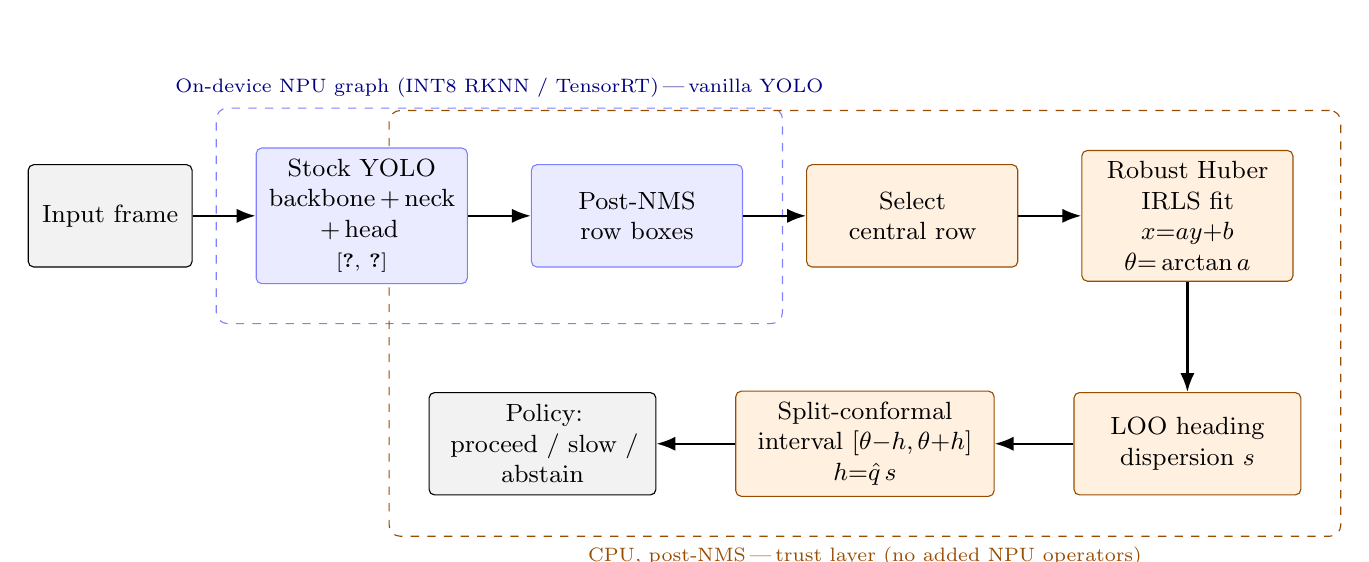
\begin{tikzpicture}[
    node distance=7mm and 8mm,
    box/.style={draw, rounded corners=2pt, align=center, font=\small,
                inner sep=4pt, minimum height=13mm, text width=24mm},
    npu/.style={box, fill=blue!8, draw=blue!50},
    cpu/.style={box, fill=orange!12, draw=orange!60!black},
    io/.style={box, fill=black!5, text width=18mm},
    flow/.style={-{Latex[length=2.4mm]}, thick},
  ]
    % ---- main forward flow (top row) ----
    \node[io]  (img)                   {Input frame};
    \node[npu, right=of img]  (det)    {Stock YOLO\\backbone\,+\,neck\\+\,head\\\scriptsize\cite{ct4,yolov10}};
    \node[npu, right=of det]  (box)    {Post-NMS\\row boxes};
    \node[cpu, right=of box]  (sel)    {Select\\central row};
    \node[cpu, right=of sel]  (fit)    {Robust Huber\\IRLS fit\\$x{=}ay{+}b$\\$\theta{=}\arctan a$};

    % ---- second row: trust layer ----
    \node[cpu, below=14mm of fit, text width=26mm] (score)
        {LOO heading\\dispersion $s$};
    \node[cpu, left=10mm of score, text width=30mm] (conf)
        {Split-conformal\\interval $[\theta{-}h,\theta{+}h]$\\$h{=}\hat q\,s$};
    \node[io, left=10mm of conf, text width=26mm] (pol)
        {Policy:\\proceed / slow /\\abstain};

    \draw[flow] (img)--(det);
    \draw[flow] (det)--(box);
    \draw[flow] (box)--(sel);
    \draw[flow] (sel)--(fit);
    \draw[flow] (fit)--(score);
    \draw[flow] (score)--(conf);
    \draw[flow] (conf)--(pol);

    % ---- grouping boxes (NPU vs CPU trust layer) ----
    \begin{scope}[on background layer]
      \node[draw=blue!50, dashed, rounded corners, fit=(det)(box),
            inner sep=5mm, label={[blue!50!black,font=\scriptsize]above:On-device NPU graph (INT8 RKNN / TensorRT)\,---\,vanilla YOLO}] {};
      \node[draw=orange!60!black, dashed, rounded corners, fit=(sel)(fit)(score)(conf)(pol),
            inner sep=5mm, label={[orange!60!black,font=\scriptsize]below:CPU, post-NMS\,---\,trust layer (no added NPU operators)}] {};
    \end{scope}
  \end{tikzpicture}}
  \caption{Know-when-to-trust crop-row guidance pipeline. A \emph{stock} YOLO detector (blue) emits
  post-NMS crop-row boxes; on the host CPU (orange) the central navigation row is selected, a robust
  Huber-IRLS line $x=ay+b$ is fit and its heading $\theta=\arctan a$ read out. The contribution is the
  trust layer: a label-free leave-one-out heading-dispersion score $s$ feeds a split-conformal
  calibration that produces a finite-sample-valid heading interval of half-width $h=\hat q\,s$, which in
  turn drives a risk-controlled proceed/slow/abstain steering policy. Everything after NMS is CPU
  arithmetic over quantities the detector already outputs, so the exported edge graph remains a vanilla
  YOLO. The detector's native DFL box-distribution variance is shown only as a non-informative negative
  control and is not used here.}
  \label{fig:pipeline}
\end{figure}


% =====================================================================
\subsection{Notation}
\label{sec:method:notation}
% =====================================================================

\noindent We use the following symbols throughout (single source of truth; no synonyms). The guidance
line is parameterised as
\begin{equation}
\label{eq:line}
x = a\,y + b ,
\end{equation}
i.e.\ image column $x$ as a function of image row $y$. This orientation is deliberate: crop rows viewed
head-on are near-vertical, so a conventional $y=mx+c$ fit becomes ill-conditioned as the slope diverges;
expressing $x$ as a function of $y$ removes this vertical-line degeneracy~\cite{sogaard}. The heading is
\begin{equation}
\label{eq:heading}
\theta = \arctan(a),
\end{equation}
reported in degrees from the vertical as the controller-independent navigation quantity, and the
cross-track offset $e_{ct}$ follows from $(a,b)$ evaluated at a look-ahead row (px; cm only under a
calibrated homography, Section~\ref{sec:setup-homography}). The detected row centroids are
$\{(x_i,y_i)\}_{i=1}^{n}$ (post-NMS box centres on the selected row). The robust line fit uses
Huber-IRLS weights $w_i$ from the Huber influence function. The nonconformity (trust) score is
$s$ = leave-one-out (LOO) heading dispersion in degrees. The held-out calibration scores are
$\{s_1,\dots,s_m\}$, split \emph{by base image}; $\hat{q}$ is the split-conformal quantile, the
$\lceil (m+1)(1-\alpha)\rceil$-th smallest of the calibration nonconformity values; the interval
half-width is $h=\hat{q}\,s$; the heading interval is $[\theta-h,\theta+h]$; $\alpha$ is the nominal
miscoverage (we report $\alpha\in\{0.10,0.05\}$); the target coverage is $1-\alpha$ and the realised
coverage is the empirical fraction of test frames whose true heading lies in the interval. The policy
thresholds are $\tau_p$ (proceed) and $\tau_s$ (slow), with abstain otherwise. The symbol
$\sigma^2_{\mathrm{DFL}}$ denotes the detector's distribution-focal-loss (DFL)~\cite{gfl} box-edge
distribution variance; it appears \emph{only} as the non-informative negative-control score in E0/E3 and
is never part of the deployed method.

% =====================================================================
\subsection{Datasets and ground truth}
\label{sec:setup-data}
% =====================================================================

\noindent\textbf{Detection labels from line ground truth.} Neither public benchmark provides bounding
boxes. CRDLD~\cite{cth1} ground truth is a binary mask of crop-row \emph{centrelines}; CRBD~\cite{crbd}
provides parametric (per-scanline) row annotations. As the detector is a stock DFL box detector, we
synthesise detection labels from the line ground truth by placing boxes on \emph{all} visible crop rows
(a single \texttt{crop\_row} segment class) at successive image rows, perspective-scaled in size.
Labelling all rows rather than only the central one avoids contradictory supervision (the rows are
visually identical), which yields a consistent, learnable target; the central navigation row is then
selected from the detections at \emph{evaluation} time (Section~\ref{sec:method:pipeline}). The box
labels are clean, so the detector still learns image difficulty rather than label noise.

\noindent\textbf{In-domain training and test: CRDLD.} The Crop Row Detection dataset of De~Silva
\textit{et~al.}~\cite{cth1} ($512\times512$; train/validation/test $=1250/250/430$) trains the detector
and serves as the in-domain test set on which the conformal coverage guarantee is evaluated under
exchangeability (E1--E4). It carries no per-field metadata, so a within-CRDLD leave-one-field-out
protocol is unavailable.

\noindent\textbf{Cross-dataset transfer: CRBD.} The Crop Row Benchmark Dataset~\cite{crbd}
($320\times240$; a different camera, crop and resolution; no training split) is a held-out
cross-dataset transfer test: the CRDLD-trained detector is evaluated on CRBD without retraining. Because
the two distributions differ, CRBD is used as a coverage-\emph{degradation} study, \emph{not} as a
setting in which the finite-sample coverage guarantee holds (Section~\ref{sec:method:conformal}).

\noindent\textbf{Field video and labelling protocol (C3).} We additionally collect and release a
diverse public crop-row \emph{field-video} dataset of real maize (forward-facing video; clips spanning
field conditions), with a hand-labelled evaluation subset of at least 100 frames. For each labelled
frame an annotator marks the central navigation row, from which the central-row line is fit in the same
$x=a\,y+b$ parameterisation~\eqref{eq:line}; inter-annotator agreement is reported in degrees
(Section~\ref{sec:setup-gtline}). The field video is uncalibrated, so its errors are reported in pixels
and degrees only, never cm; it is used as a second cross-distribution coverage-degradation probe (E2,
E5) and as the ordered frame sequence for the open-loop policy replay (E6). Frames from the same clip
are kept together when splitting, to respect the exchangeability assumption as far as the data allow.

\noindent The CRDLD train/validation/test splits are disjoint, CRBD is an entirely separate dataset, and
the field video is recorded independently, so memorisation cannot inflate any transfer or coverage
result. Table~\ref{tab:setup-datasets} summarises the role of each dataset. A Data and Code Availability
statement accompanies the manuscript.

\begin{table}[!ht]
\centering
\caption{Datasets and their role. Boxes are synthesised from the line ground truth
(Section~\ref{sec:setup-data}); the evaluation ground-truth line is annotation/mask-derived and
detector-independent. cm units are reported only where the camera is calibrated. \emph{Results to be
completed.}}
\label{tab:setup-datasets}
\resizebox{\columnwidth}{!}{\begin{tabular}{lllc}
\hline
\textbf{Dataset} & \textbf{Role} & \textbf{GT guidance line} & \textbf{cm scale?} \\
\hline
CRDLD~\cite{cth1} ($512^2$; 1250/250/430) & Train detector $+$ in-domain coverage & line-mask $\rightarrow$ central row & calibrated \\
CRBD~\cite{crbd} ($320{\times}240$) & Cross-dataset coverage-degradation & annotation $\rightarrow$ central row & px/deg \\
Field video (maize; $\geq$100 labelled) & Coverage-degradation $+$ E6 replay & hand-labelled central row & px/deg \\
\hline
\end{tabular}}
\end{table}

% =====================================================================
\subsection{Pixel-to-centimetre calibration}
\label{sec:setup-homography}
% =====================================================================

\noindent Because ``cm'' is meaningless without a metric anchor, we report centimetres only where the
camera is calibrated (the robot platform and the CRDLD homography), and pixels/degrees everywhere else.
Where camera intrinsics and extrinsics (or a checkerboard reference) are available, we recover the
image-to-ground homography $H$ under an explicit \emph{flat-ground assumption} and report it; the
projection $H$ is applied to line samples to obtain cross-track in cm. Otherwise --- including the field
video --- we report errors in pixels and in pixels normalised by image width, and do not invent a
centimetre value. Flat ground is stated as an explicit limitation with an error budget: a camera-pitch
perturbation propagates to a look-ahead-distance error that grows with range, so we tabulate the induced
centimetre error at the look-ahead row as a function of pitch, making the conditions under which the
centimetre numbers are trustworthy auditable.

% =====================================================================
\subsection{Frozen ground-truth guidance-line extraction}
\label{sec:setup-gtline}
% =====================================================================

\noindent The ground-truth (GT) guidance line used for \emph{evaluation} is derived from the
segmentation mask / annotation and is therefore detector-independent. The extraction is frozen as
follows (\texttt{gt\_line\_from\_mask}). For each crop-row mask we compute, per image row $y$, the
median column $x$ of foreground pixels, then fit a robust Huber-IRLS regression to those per-row
medians, selecting as the navigation row the one nearest the image-centre-bottom; gap and occlusion
handling are part of the frozen procedure. The resulting line is expressed in the same $x=a\,y+b$
parameterisation~\eqref{eq:line}, with heading $\theta=\arctan(a)$~\eqref{eq:heading}. To validate the
auto-extracted GT we cross-check it against a human-annotated subset of at least 100 frames and report
inter-annotator agreement in degrees (and cm where the homography permits), in
Table~\ref{tab:setup-gtline}. The GT line is mask/annotation-derived, not a least-squares fit through GT
box centroids, so it is independent of the box-synthesis step of Section~\ref{sec:setup-data}.

\begin{table}[!ht]
\centering
\caption{Frozen GT-line extraction: agreement between the automatic mask-derived line and human
annotation on the cross-check subset ($\geq$100 frames). cm reported only on the calibrated platform.
\emph{Results to be completed.}}
\label{tab:setup-gtline}
\begin{tabular}{lcc}
\hline
\textbf{Quantity} & \textbf{Heading ($^\circ$)} & \textbf{Cross-track (cm)} \\
\hline
Auto vs.\ human (median $|\Delta|$) & -- & -- \\
Inter-annotator (median $|\Delta|$) & -- & -- \\
\hline
\end{tabular}
\end{table}

% =====================================================================
\subsection{The guidance pipeline: detect, select, robust fit}
\label{sec:method:pipeline}
% =====================================================================

\noindent\textbf{Detect.} Given a forward-facing field image, the stock detector returns crop-row
segment boxes after non-maximum suppression (NMS). For box $i$ we take its centroid $(x_i,y_i)$ in
pixels (\texttt{detect\_with\_logits} $\rightarrow$ \texttt{guidance\_line} in \texttt{eval\_guidance.py}).
The detector fires on \emph{all} rows by design.

\noindent\textbf{Select the central row.} A single guidance line is fit through the centroids of the
\emph{central} navigation row. We seed at the bottom-centre detection, estimate a local slope from the
bottom-most boxes near the seed, and keep detections within a fixed image-fraction corridor of the
\emph{predicted} central-row line $a_{\mathrm{seed}}\,y + b_{\mathrm{seed}}$ (\texttt{select\_central}).
Selecting against the predicted line rather than walking from box to box prevents the reference from
drifting onto an adjacent row, which would leak wrong-row outliers into the fit --- the dominant failure
mode this paper's trust score is designed to catch.

\noindent\textbf{Robust Huber-IRLS line fit (deployed).} Given the $n$ selected centroids, the deployed
guidance line solves a Huber robust regression of $x$ on $y$,
\begin{equation}
\label{eq:irls_obj}
(\hat a,\hat b) = \arg\min_{a,b}\; \sum_{i=1}^{n} \rho_\delta\!\bigl(x_i - a\,y_i - b\bigr),
\qquad
\rho_\delta(r) =
\begin{cases}
\tfrac{1}{2}r^2, & |r|\le\delta,\\[2pt]
\delta\bigl(|r|-\tfrac{1}{2}\delta\bigr), & |r|>\delta,
\end{cases}
\end{equation}
solved by iteratively reweighted least squares (IRLS): at each iteration the residuals
$r_i = x_i-\hat a\,y_i-\hat b$ are rescaled by a robust scale $\hat\sigma = 1.4826\,\mathrm{median}_i|r_i|$
and the Huber influence weights
\begin{equation}
\label{eq:huber_w}
w_i = \min\!\left(1,\ \frac{\delta\,\hat\sigma}{|r_i|}\right),
\qquad \delta = 1.345,
\end{equation}
are applied in a weighted least-squares solve of $x=a\,y+b$; a small per-diagonal ridge keeps the
normal equations well-conditioned (the intercept and slope entries differ by orders of magnitude). The
weights $w_i$ are the \emph{Huber} weights of Equation~\eqref{eq:huber_w} --- robustness to wrong-row
contamination --- and are \emph{not} DFL precision weights. We verified that the detector's native DFL
box-distribution variance $\sigma^2_{\mathrm{DFL}}$ is non-informative for heading error in this setting
(Spearman $\rho=-0.13$; reported as the E0 negative control, Section~\ref{sec:res-e0-trustinfo}), so
robustness, not variance weighting, is what works. This robust readout matches a RANSAC baseline and far
exceeds equal-weight least squares (C1, E1).

\noindent\textbf{Baseline and ablation readouts.} The harness exposes six readouts sharing one stock
checkpoint, so they are compared paired per frame: \texttt{equalLS} (non-robust equal-weight LS, the
detect-then-fit recipe of~\cite{diao_yolox}); \texttt{ransac} (robust consensus LS, a strong baseline);
\texttt{irls} (the deployed Huber-IRLS, equal data weights); \texttt{calm} (the dead DFL-precision
$\times$ Huber-IRLS variant, retained only as a negative control --- it is \emph{not} the
contribution); \texttt{qual} (detector-confidence-squared weights); and \texttt{oracle} (weights from
the true residual to the GT line, an upper bound). Heading error is
$|\arctan(\hat a)-\arctan(a_{\mathrm{gt}})|$ and line-fit RMSE is sampled over $y$ \emph{including} the
far look-ahead row (\texttt{heading\_err\_deg}, \texttt{line\_rmse\_px}).

% =====================================================================
\subsection{Label-free trust score: leave-one-out heading dispersion}
\label{sec:method:score}
% =====================================================================

\noindent The trust score must be \emph{label-free} (computable at run time without ground truth) and
\emph{matched to the failure mode} (wrong-row contamination, which inflates heading error). We use
leave-one-out (LOO) heading dispersion (\texttt{loo\_heading\_dispersion}). For each of the $n$ central
centroids, we refit the guidance line with that centroid removed and record the resulting heading
$\theta^{(-i)}=\arctan(\hat a^{(-i)})$; the nonconformity score is the dispersion of these LOO headings,
\begin{equation}
\label{eq:loo_score}
s = \operatorname{std}_{i=1,\dots,n}\!\bigl(\theta^{(-i)}\bigr)\ \ (\text{deg}).
\end{equation}
A high $s$ means the heading hinges on a single detection --- a wrong-row outlier, or too few /
ill-conditioned points --- and should not be trusted; a low $s$ means the heading is geometrically
stable. This score directly targets the measured failure mode, unlike $\sigma^2_{\mathrm{DFL}}$. As
candidate alternatives for the sharpness ablation (E3) the harness also logs: the robust residual scale
of the fit, $1-$inlier-fraction, $1-$mean detection confidence, the mean DFL centroid sigma
($\sigma_{\mathrm{DFL}}$, the dead control), and $1/\sqrt{n}$ (\texttt{s\_resid}, \texttt{s\_inv\_inlier},
\texttt{s\_conf}, \texttt{s\_dfl}, \texttt{s\_ninv}). The mean detection confidence is also retained as
the score for the fixed-confidence baseline gate (E4).

% =====================================================================
\subsection{Split-conformal heading intervals}
\label{sec:method:conformal}
% =====================================================================

\noindent We turn the score $s$ into a finite-sample-valid heading prediction interval via
\emph{normalised (score-scaled) split conformal}~\cite{vovk2005,lei2018,romano2019cqr} (\texttt{conformal.py}).
On a held-out calibration set of $m$ frames we form the normalised residuals
\begin{equation}
\label{eq:conf_R}
R_j = \frac{|\theta_j - \theta_j^{\mathrm{gt}}|}{s_j}, \qquad j=1,\dots,m,
\end{equation}
and take the split-conformal quantile
\begin{equation}
\label{eq:conf_qhat}
\hat q = R_{(k)},\qquad k = \bigl\lceil (m+1)(1-\alpha)\bigr\rceil,
\end{equation}
the $k$-th smallest of $\{R_j\}$ (\texttt{calibrate}). For a test frame with heading $\theta$ and score
$s$ the interval is $[\theta-h,\theta+h]$ with half-width
\begin{equation}
\label{eq:conf_hw}
h = \hat q\,s
\end{equation}
(\texttt{half\_width}). The constant-width conformal baseline sets $s\equiv 1$.

\noindent\textbf{Coverage statement and exchangeability (honest).} Under \emph{exchangeability of the
calibration and test scores within one distribution}, split conformal guarantees the finite-sample
bound $\Pr\!\bigl(|\theta-\theta^{\mathrm{gt}}|\le \hat q\,s\bigr)\ge 1-\alpha$, i.e.\ realised coverage
$\ge 1-\alpha$ in expectation over the calibration draw~\cite{vovk2005,lei2018}. This guarantee holds
on the in-domain CRDLD test (E2), where we split \emph{by base image} to keep frames from the same scene
out of both calibration and test. It does \emph{not} transfer to CRBD or the field video, whose
distributions differ; for those we report realised coverage as a \emph{coverage-degradation study},
explicitly not a guarantee, and we state this every time coverage is claimed. Realised coverage is
reported with Clopper--Pearson (and Wilson) confidence intervals (\texttt{clopper\_pearson},
\texttt{wilson\_ci}), marginally and stratified by difficulty.

% =====================================================================
\subsection{Risk-controlled steering policy and open-loop replay}
\label{sec:method:policy}
% =====================================================================

\noindent\textbf{Abstain/slow/proceed.} The certified half-width $h=\hat q\,s$ drives a three-way
steering policy: \emph{proceed} if $h\le\tau_p$, \emph{slow} if $\tau_p<h\le\tau_s$, and \emph{abstain}
(stop / hold the last trusted heading) if $h>\tau_s$. Sweeping the threshold traces a selective-risk
curve --- heading error on \emph{accepted} frames versus abort (abstain) rate
(\texttt{selective\_risk}). We compare it against the fixed-confidence baseline gate that accepts a frame
iff the mean detection confidence exceeds a threshold (\texttt{selective\_risk\_fixed}), at matched abort
rate, and we frame the policy as risk-controlled in the sense of distribution-free risk
control~\cite{angelopoulos2022rcps} and selective prediction with a reject option~\cite{geifman2017selective}.

\noindent\textbf{Open-loop kinematic-bicycle replay (honest, E6).} We have no field-robot odometry, so
E6 is explicitly an \emph{open-loop policy replay}, not a closed-loop field result. Over an ordered
frame sequence we feed the per-frame heading command through one kinematic-bicycle / pure-pursuit
step~\cite{rajamani2012} and accumulate a lateral-deviation surrogate (\texttt{bicycle\_replay} /
\texttt{simulate\_cross\_track}); under the abstain policy the controller holds the last trusted heading
instead of acting on an untrusted (possibly wrong-row) estimate. We report the integrated lateral
deviation and the count of large-heading-error accepted commands for the conformal policy versus a fixed
threshold; the claim is only that the abstain rule reduces large-error commands, stated as an open-loop
replay.

% =====================================================================
\subsection{Edge deployment}
\label{sec:setup-edge}
% =====================================================================

\noindent The detector is deployed on two edge platforms (Table~\ref{tab:setup-edge}): TensorRT
(FP16 and INT8) on an NVIDIA Jetson Nano~\cite{tensorrt}, and RKNN INT8 on a Rockchip
NPU~\cite{rknntoolkit}, with post-training INT8 quantization following standard integer-arithmetic
inference~\cite{jacob2018int8}. For each we report latency (mean\,$\pm$\,std and P95), throughput (FPS),
and input resolution. Because the trust layer is CPU post-NMS arithmetic over quantities the detector
already outputs, it adds no operators to the exported NPU graph, so the exported detector is a vanilla
YOLO and the on-device cost is the detector's alone; structural pruning~\cite{cth14,ct17} and efficient
backbones~\cite{ct16,ct19} are optional efficiency levers reported on the same axes if applied.
Critically, we re-fit the conformal quantile $\hat q$ \emph{after} INT8 conversion on a small
calibration set and verify that realised coverage survives quantization (E5), since INT8 perturbs the
detected centroids and hence the scores.

\begin{table}[!ht]
\centering
\caption{Edge deployment on the two named platforms. The trust layer adds no NPU operators; the
exported graph is a vanilla YOLO. \emph{Results to be completed.}}
\label{tab:setup-edge}
\resizebox{\columnwidth}{!}{\begin{tabular}{llcccc}
\hline
\textbf{Platform} & \textbf{Precision} & \textbf{Latency mean$\pm$std (ms)} & \textbf{P95 (ms)} & \textbf{FPS} & \textbf{Coverage post-INT8} \\
\hline
Jetson Nano (TensorRT) & FP16 & -- & -- & -- & -- \\
Jetson Nano (TensorRT) & INT8 & -- & -- & -- & -- \\
Rockchip (RKNN) & INT8 & -- & -- & -- & -- \\
\hline
\end{tabular}}
\end{table}

% =====================================================================
\subsection{Evaluation protocol, metrics, and statistics}
\label{sec:setup-metrics}
% =====================================================================

\noindent\textbf{Metrics.} The primary metric is heading error in degrees (controller-independent).
Line-fit RMSE is reported in pixels (and cm where the homography of Section~\ref{sec:setup-homography}
permits), evaluated \emph{including} the look-ahead row. Cross-track is a static geometric proxy: the
lateral offset between the predicted and GT lines at the look-ahead row (px, and cm where calibrated).
For the conformal layer we report realised vs.\ nominal coverage at $\alpha\in\{0.10,0.05\}$ and interval
\emph{width} (sharpness, deg) at matched coverage. For the policy we report heading error on accepted
frames and the large-heading-error rate ($>5^\circ$) versus abort rate. Detection mAP@50 and mAP@50--95
are secondary diagnostics; edge latency/throughput are reported on the named devices
(Section~\ref{sec:setup-edge}).

\noindent\textbf{Statistical protocol.} The evaluation script (\texttt{eval\_guidance.py}) writes one
CSV row per frame so that the shared-checkpoint readout arms are compared \emph{paired}, and
\texttt{eval\_conformal.py} runs the conformal experiments on those CSVs. Point-accuracy comparisons
(E1) use $\geq 5$ seeds; because $n$ is small for normality, significance uses the paired
\emph{Wilcoxon signed-rank} test with \emph{Holm--Bonferroni} correction across the confirmatory family,
and we report \emph{Cliff's $\delta$} effect sizes with 95\% bootstrap confidence intervals, not merely
$p<0.05$. Coverage proportions are reported with \emph{Clopper--Pearson} (and Wilson) confidence
intervals. The calibration/test split is by base image on CRDLD and by clip on the field video to
respect exchangeability; any claim whose $\Delta$ is smaller than its standard deviation is downgraded in
wording.

\noindent\textbf{Experiment map (E0--E6).} The protocol is organised into seven experiments, reported in
Section~\ref{sec:results}: \textbf{E0} trust-score informativeness --- Spearman $\rho(s,\text{realised
heading error})>0$, with $\sigma^2_{\mathrm{DFL}}$ ($\rho=-0.13$) as the negative control
(Section~\ref{sec:res-e0-trustinfo}); \textbf{E1} point-accuracy floor --- heading error for
equalLS/ransac/irls(deployed)/calm/qual/oracle on CRDLD test, $\geq 5$ seeds, paired Wilcoxon $+$ Holm
$+$ Cliff's $\delta$ (Section~\ref{sec:res-e1-accuracy}); \textbf{E2} coverage --- realised vs.\ nominal
at $\alpha\in\{0.10,0.05\}$, Clopper--Pearson CIs, marginal and by difficulty, split by base image
(Section~\ref{sec:res-e2-coverage}); \textbf{E3} sharpness / score-ablation --- interval width at matched
coverage for $s$ vs.\ residual vs.\ $\mathrm{conf}^2$ vs.\ $\sigma_{\mathrm{DFL}}$ vs.\
RANSAC-consensus, where the proposed score should be tightest (Section~\ref{sec:res-e3-sharpness});
\textbf{E4} selective-risk --- error on accepted frames vs.\ abort rate, conformal-width gate vs.\ the
fixed-confidence gate at matched abort (Section~\ref{sec:res-e4-selrisk}); \textbf{E5} deployment ---
Jetson/TensorRT and RKNN INT8 latency/FPS and coverage-survives-INT8 (Section~\ref{sec:res-e5-deploy});
and \textbf{E6} open-loop kinematic-bicycle policy replay (Section~\ref{sec:res-e6-replay}).

%!TEX root = ../main.tex

\section{Results}
\label{sec:results}

This section reports the empirical evaluation of the proposed trust layer --- a
split-conformal heading-interval and risk-controlled steering policy bolted onto
a \emph{stock} detector (YOLOv8n) with a robust Huber-IRLS line fit. \emph{No
dataset-level numbers are filled in yet}: every quantitative cell is a
placeholder (``\texttt{--}'' in tables, ``[TODO]'' in prose) to be completed once
the pre-registered runs (experiments E0--E6) have finished. The table
structures, comparison arms, metrics, statistical tests, and pass criteria below
are fixed in advance so that the analysis is confirmatory rather than
exploratory. Each table and figure is wrapped in \verb|\IfFileExists| so the
manuscript compiles today; the auto-generated file is \verb|\input| once a run
produces it.

We restate the readout so the tables are self-contained. From the post-NMS box
centroids $\{(x_i,y_i)\}_{i=1}^{n}$ we fit the guidance line $x = a\,y + b$ by
robust Huber-IRLS, with weights $w_i$ from the Huber influence function; the
heading is $\theta = \arctan(a)$ in degrees from vertical and the cross-track
offset is $e_{ct}$ (px, or cm only under the calibrated homography of
Section~\ref{sec:setup-homography}). This readout adds no NPU operators because
it is CPU math executed after NMS; the exported detector graph is a vanilla YOLO.
The trust score is the leave-one-out (LOO) heading dispersion $s$ (deg): the
dispersion of $\theta$ over refits that each omit one centroid, which targets
wrong-row contamination without any extra labels. Split-conformal calibration on
a held-out score set $\{s_1,\dots,s_m\}$ (split \emph{by base image}) gives the
quantile $\hat q$, and the heading interval is $[\theta - h, \theta + h]$ with
half-width $h = \hat q\,s$, locally adaptive in the sense of conformalized
quantile regression~\cite{romano2019cqr,lei2018,vovk2005,angelopoulos2023}. We
report nominal miscoverage $\alpha\in\{0.10,0.05\}$ and the realised coverage,
with Clopper--Pearson / Wilson intervals. Throughout, the detector's native DFL
box-edge distribution variance $\sigma^2_{\mathrm{DFL}}$~\cite{gfl,gflv2} appears
\emph{only} as a non-informative negative control; the deployed line fit is
robust Huber-IRLS, not variance weighting.

\paragraph{Scope and honesty caveats.} Three caveats bound every claim below.
(i)~This is an \emph{applied} contribution --- a trust layer and evaluation on a
stock detector --- not a new detector architecture. (ii)~The conformal coverage
guarantee is finite-sample-valid only \emph{under exchangeability within one
distribution}; results on CRBD and on field video are therefore a
coverage-\emph{degradation} study, not a guarantee, and are labelled as such
wherever coverage is reported. (iii)~The policy replay (E6) is an
\emph{open-loop} kinematic-bicycle replay~\cite{rajamani2012}, not a closed-loop
field-robot run: no odometry is in the loop, so E6 measures how the abstain
policy would have filtered large-heading-error frames, not realised tracking
error. Centimetre units are used only where the camera is calibrated (the robot
platform and the CRDLD homography); field video stays in px and deg.

\subsection{E0 --- Is the trust score informative? (and the DFL-variance negative control)}
\label{sec:res-e0-trustinfo}

E0 tests the premise of the whole trust layer: that the LOO dispersion score $s$
actually tracks the realised heading error, frame by frame. Table~\ref{tab:e0-trustinfo}
reports the Spearman rank correlation $\rho(s,\,|\theta-\theta^\star|)$ between
the score and the realised heading error on CRDLD test (split by base image,
$\ge 5$ seeds), with a bootstrap CI. The pass criterion is $\rho > 0$ with a CI
excluding zero: a positive, significant correlation is what licenses using $s$
as a nonconformity score in E2--E4. The same table reports, as a \emph{negative
control}, the rank correlation of the detector's native DFL box-edge variance
$\sigma^2_{\mathrm{DFL}}$~\cite{gfl,gflv2} with the identical error target; our
prior measurement on this data is $\rho_{\mathrm{DFL}} = -0.13$, i.e.\
non-informative (and, if anything, anti-correlated). This contrast is the
empirical reason the deployed readout uses robust Huber-IRLS rather than
DFL-variance precision weighting: the box-distribution variance does not track
heading reliability here. Figure~\ref{fig:e0-scatter} visualises both
relationships as score-versus-error scatters.

\IfFileExists{tables/tab_e0.tex}{\input{tables/tab_e0.tex}}{%
{\renewcommand{\arraystretch}{1.3}
\begin{table}[!ht]
  \centering
  \caption{E0 --- Trust-score informativeness on CRDLD test, split by base
    image, $\ge 5$ seeds. Spearman $\rho$ between each candidate score and the
    realised heading error $|\theta-\theta^\star|$, with bootstrap 95\,\% CIs.
    The proposed LOO-dispersion score $s$ must satisfy $\rho>0$ (CI excluding
    zero); the DFL-variance row $\sigma^2_{\mathrm{DFL}}$ is the non-informative
    negative control. \emph{Results to be completed.}}
  \label{tab:e0-trustinfo}
  \resizebox{\columnwidth}{!}{\begin{tabular}{lcccc}
    \hline
    \textbf{Candidate score} & \textbf{Spearman $\rho$} & \textbf{95\,\% CI} & \textbf{$\rho>0$?} & \textbf{Role} \\
    \hline
    $s$ = LOO heading dispersion        & -- & [--,\,--] & -- & proposed \\
    Fit residual (median)               & -- & [--,\,--] & -- & alt.\ score \\
    Detector confidence$^2$             & -- & [--,\,--] & -- & alt.\ score \\
    RANSAC consensus fraction           & -- & [--,\,--] & -- & alt.\ score \\
    $\sigma^2_{\mathrm{DFL}}$ (DFL var) & -- & [--,\,--] & -- & negative control \\
    \hline
  \end{tabular}}
  \medskip
\end{table}}%
}

\IfFileExists{figures/fig_e0_scatter.pdf}{%
\begin{figure}[!ht]\centering
\includegraphics[width=0.72\linewidth]{figures/fig_e0_scatter.pdf}
\caption{E0 --- Realised heading error versus candidate trust score on CRDLD
  test: the proposed LOO-dispersion score $s$ (informative) contrasted with the
  DFL box-edge variance $\sigma^2_{\mathrm{DFL}}$ (non-informative negative
  control). \emph{Auto-generated from the run.}}\label{fig:e0-scatter}
\end{figure}}{}

\subsection{E1 --- Point-accuracy floor of the guidance readout}
\label{sec:res-e1-accuracy}

E1 establishes the point-heading accuracy floor: before any interval is claimed,
the deployed Huber-IRLS readout must produce a competitive point heading.
Table~\ref{tab:e1-accuracy} reports heading error (deg) on CRDLD test ($\ge 5$
seeds), and line-fit RMSE (px, and cm under the calibrated homography), for six
readout arms that all share a single stock YOLOv8n checkpoint and differ only in
the CPU-side line fit: equal-weight least squares (\textbf{equalLS}, the
Diao-style detect-then-fit recipe~\cite{diao_yolox}), \textbf{RANSAC} least
squares, the deployed robust \textbf{IRLS} (Huber), the dead DFL-variance
precision-weighted variant (\textbf{CALM}, included only as the negative control
of E0/E3), a qualitative single-frame heuristic (\textbf{qual}), and an
\textbf{oracle} that picks the best-of-arm per frame (an upper bound, not a
deployable method). Because the arms are paired per frame, comparisons use the
Wilcoxon signed-rank test with Holm correction across the confirmatory family
and Cliff's $\delta$ as effect size. The pre-registered claims are: IRLS
\emph{matches} RANSAC (no significant difference, or $|\delta|<0.147$) and IRLS
\emph{far beats} equalLS (Holm-adjusted $p<0.05$ and $|\delta|\ge 0.33$), with
median heading sub-degree. We also report cross-dataset transfer (CRDLD
$\leftrightarrow$ CRBD~\cite{crbd,cth1,cth2}) so the floor is not a single-domain
artefact. Figure~\ref{fig:e1-box} shows the per-arm heading-error distribution,
and Figure~\ref{fig:qual-lines} shows qualitative fits.

\IfFileExists{tables/tab_e1.tex}{\input{tables/tab_e1.tex}}{%
{\renewcommand{\arraystretch}{1.3}
\begin{table}[!ht]
  \centering
  \caption{E1 --- Point-accuracy floor on CRDLD test, mean$\pm$std over $\ge 5$
    seeds; cm only under the calibrated homography (Section~\ref{sec:setup-homography}).
    All arms share one stock YOLOv8n checkpoint and differ only in the post-NMS
    line fit. Pairwise tests vs.\ the deployed IRLS arm: Wilcoxon signed-rank,
    Holm-adjusted, Cliff's $\delta$. \texttt{calm}=DFL-variance weighting
    (negative control); \texttt{oracle}=best-of-arm upper bound (not
    deployable). \emph{Results to be completed.}}
  \label{tab:e1-accuracy}
  \resizebox{\columnwidth}{!}{\begin{tabular}{lccccc}
    \hline
    \textbf{Readout arm} & \textbf{Heading ($^\circ$)$\downarrow$} & \textbf{RMSE (px)$\downarrow$} & \textbf{RMSE (cm)$\downarrow$} & \textbf{Wilcoxon $p$ (Holm)} & \textbf{Cliff's $\delta$} \\
    \hline
    equalLS~\cite{diao_yolox}        & -- & -- & -- & -- & -- \\
    RANSAC                           & -- & -- & -- & -- & -- \\
    \textbf{IRLS (deployed, Huber)}  & -- & -- & -- & \emph{ref} & \emph{ref} \\
    calm (DFL-var, neg.\ control)    & -- & -- & -- & -- & -- \\
    qual (single-frame heuristic)    & -- & -- & -- & -- & -- \\
    oracle (best-of-arm, upper bound)& -- & -- & -- & -- & -- \\
    \hline
  \end{tabular}}
  \medskip
\end{table}}%
}

\IfFileExists{figures/fig_e1_box.pdf}{%
\begin{figure}[!ht]\centering
\includegraphics[width=0.62\linewidth]{figures/fig_e1_box.pdf}
\caption{E1 --- Per-arm heading-error distribution on CRDLD test ($\ge 5$
  seeds). Boxes show median and IQR; the deployed IRLS arm is highlighted.
  \emph{Auto-generated from the run.}}\label{fig:e1-box}
\end{figure}}{}

\IfFileExists{figures/fig_qualitative.pdf}{%
\begin{figure}[!ht]\centering
\includegraphics[width=0.92\linewidth]{figures/fig_qualitative.pdf}
\caption{Qualitative guidance lines on CRDLD test frames: ground-truth line
  (green) vs.\ the deployed Huber-IRLS fit (red) over detected row-segment
  centroids, with the conformal heading interval shaded.
  \emph{Auto-generated from the run.}}\label{fig:qual-lines}
\end{figure}}{}

\subsection{E2 --- Realised vs.\ nominal coverage}
\label{sec:res-e2-coverage}

E2 is the central validity check for the trust layer. Table~\ref{tab:e2-coverage}
reports the realised coverage --- the empirical fraction of test frames whose
true heading lies in $[\theta-h,\theta+h]$ --- against the nominal target
$1-\alpha$ for $\alpha\in\{0.10,0.05\}$, with Clopper--Pearson and Wilson 95\,\%
CIs. Calibration and test are split \emph{by base image} so that exchangeability
is not broken by near-duplicate frames; this split is what makes the
split-conformal coverage guarantee~\cite{vovk2005,lei2018,angelopoulos2023}
applicable in-domain. The pass criterion is that the realised-coverage CI
contains the nominal target on the CRDLD in-domain test (marginal coverage), and
we additionally report coverage stratified by difficulty (near/far rows, low/high
centroid count) to expose conditional under-coverage. Cross-dataset rows
(CRDLD$\to$CRBD and field video~\cite{crbd,cth2}) are reported as a
coverage-\emph{degradation} study: exchangeability does not hold across
distributions, so any shortfall there quantifies how far the in-domain guarantee
travels, and is \emph{not} a claimed guarantee. Figure~\ref{fig:e2-reliability}
is the reliability diagram (realised vs.\ nominal across a sweep of $\alpha$).
We position this as a domain instantiation of conformal prediction on a detector
and explicitly contrast, rather than claim primacy over, prior
conformal-on-detector work~\cite{confdet1,confdet2}.

\IfFileExists{tables/tab_e2.tex}{\input{tables/tab_e2.tex}}{%
{\renewcommand{\arraystretch}{1.3}
\begin{table}[!ht]
  \centering
  \caption{E2 --- Realised vs.\ nominal heading-interval coverage, split by base
    image, with Clopper--Pearson / Wilson 95\,\% CIs. CRDLD is the in-domain
    guarantee (CI should contain $1-\alpha$); CRDLD$\to$CRBD and field video are
    a coverage-\emph{degradation} study under distribution shift (not a
    guarantee). \emph{Results to be completed.}}
  \label{tab:e2-coverage}
  \resizebox{\columnwidth}{!}{\begin{tabular}{llcccc}
    \hline
    \textbf{Eval set} & \textbf{$\alpha$} & \textbf{Nominal $1-\alpha$} & \textbf{Realised} & \textbf{Clopper--Pearson CI} & \textbf{In CI?} \\
    \hline
    \multirow{2}{*}{CRDLD (in-domain)}
      & 0.10 & 0.90 & -- & [--,\,--] & -- \\
      & 0.05 & 0.95 & -- & [--,\,--] & -- \\
    \hline
    \multirow{2}{*}{CRDLD$\to$CRBD (shift)}
      & 0.10 & 0.90 & -- & [--,\,--] & -- \\
      & 0.05 & 0.95 & -- & [--,\,--] & -- \\
    \hline
    \multirow{2}{*}{Field video (shift)}
      & 0.10 & 0.90 & -- & [--,\,--] & -- \\
      & 0.05 & 0.95 & -- & [--,\,--] & -- \\
    \hline
  \end{tabular}}
  \medskip
\end{table}}%
}

\IfFileExists{figures/fig_e2_reliability.pdf}{%
\begin{figure}[!ht]\centering
\includegraphics[width=0.55\linewidth]{figures/fig_e2_reliability.pdf}
\caption{E2 --- Reliability diagram: realised vs.\ nominal heading-interval
  coverage over a sweep of $\alpha$, CRDLD in-domain (on the diagonal under
  exchangeability) with the distribution-shift sets shown as a degradation
  study. \emph{Auto-generated from the run.}}\label{fig:e2-reliability}
\end{figure}}{}

\subsection{E3 --- Sharpness: which score gives the tightest valid interval?}
\label{sec:res-e3-sharpness}

A trust layer is useful only if its valid intervals are also \emph{sharp}: wide
intervals that always cover are uninformative for steering. E3 ablates the
nonconformity score, holding the conformal machinery and the target coverage
fixed, and reports the mean interval half-width $h$ at matched realised coverage.
Table~\ref{tab:e3-sharpness} compares the proposed LOO-dispersion score $s$
against the fit residual, the squared detector confidence, the DFL box-edge
variance $\sigma^2_{\mathrm{DFL}}$~\cite{gfl,gflv2}, and the RANSAC consensus
fraction. Because all scores are conformalized to the same $1-\alpha$, coverage
is (by construction) matched and the discriminating axis is width: the
pre-registered claim is that the failure-mode-matched LOO-dispersion score yields
the \emph{narrowest} mean half-width at matched coverage, with the
non-informative DFL-variance score giving the widest. Figure~\ref{fig:e3-width}
plots the half-width distribution per score.

\IfFileExists{tables/tab_e3.tex}{\input{tables/tab_e3.tex}}{%
{\renewcommand{\arraystretch}{1.3}
\begin{table}[!ht]
  \centering
  \caption{E3 --- Interval sharpness (score ablation) on CRDLD test, split by
    base image, $\ge 5$ seeds, at matched realised coverage ($\alpha=0.10$).
    Mean conformal half-width $h$ (deg, lower is sharper); realised coverage
    column confirms the comparison is at matched coverage. The proposed
    LOO-dispersion score $s$ should be tightest; $\sigma^2_{\mathrm{DFL}}$
    widest. \emph{Results to be completed.}}
  \label{tab:e3-sharpness}
  \resizebox{\columnwidth}{!}{\begin{tabular}{lccc}
    \hline
    \textbf{Nonconformity score} & \textbf{Realised coverage} & \textbf{Mean half-width $h$ ($^\circ$)$\downarrow$} & \textbf{Rank} \\
    \hline
    $s$ = LOO heading dispersion        & -- & -- & -- \\
    Fit residual                        & -- & -- & -- \\
    Detector confidence$^2$             & -- & -- & -- \\
    $\sigma^2_{\mathrm{DFL}}$ (DFL var) & -- & -- & -- \\
    RANSAC consensus fraction           & -- & -- & -- \\
    \hline
  \end{tabular}}
  \medskip
\end{table}}%
}

\IfFileExists{figures/fig_e3_width.pdf}{%
\begin{figure}[!ht]\centering
\includegraphics[width=0.62\linewidth]{figures/fig_e3_width.pdf}
\caption{E3 --- Conformal half-width distribution per nonconformity score at
  matched coverage on CRDLD test; narrower is sharper.
  \emph{Auto-generated from the run.}}\label{fig:e3-width}
\end{figure}}{}

\subsection{E4 --- Selective risk: does the conformal gate beat a confidence gate?}
\label{sec:res-e4-selrisk}

E4 evaluates the steering policy as a selective predictor~\cite{geifman2017selective,angelopoulos2022rcps}:
frames are accepted (proceed) or aborted (abstain), and we plot the heading error
on \emph{accepted} frames against the abort rate. Table~\ref{tab:e4-selrisk}
compares the conformal-width gate (abstain when the half-width $h$ exceeds a
threshold) against the fixed-confidence baseline gate (abstain when detector
confidence is below a threshold), at \emph{matched abort rate} so the comparison
is fair. The pre-registered claim is that, at matched abort, the conformal-width
gate yields lower heading error on accepted frames --- i.e.\ it aborts the right
frames --- because it is driven by a failure-mode-matched score rather than by
raw confidence. Figure~\ref{fig:e4-riskcov} is the risk--coverage curve (accepted
error vs.\ abort rate) for both gates; a uniformly lower conformal curve is the
visual statement of the same claim.

\IfFileExists{tables/tab_e4.tex}{\input{tables/tab_e4.tex}}{%
{\renewcommand{\arraystretch}{1.3}
\begin{table}[!ht]
  \centering
  \caption{E4 --- Selective risk on CRDLD test, split by base image, $\ge 5$
    seeds. Heading error on accepted frames at matched abort rate: conformal-width
    gate vs.\ fixed-confidence gate. Lower accepted error at equal abort is
    better. \emph{Results to be completed.}}
  \label{tab:e4-selrisk}
  \resizebox{\columnwidth}{!}{\begin{tabular}{lcccc}
    \hline
    \textbf{Abort rate} & \textbf{Conf-gate error ($^\circ$)$\downarrow$} & \textbf{Conformal-gate error ($^\circ$)$\downarrow$} & \textbf{$\Delta$ ($^\circ$)} & \textbf{Better} \\
    \hline
    0\,\% (no abstain) & -- & -- & -- & -- \\
    5\,\%              & -- & -- & -- & -- \\
    10\,\%             & -- & -- & -- & -- \\
    20\,\%             & -- & -- & -- & -- \\
    \hline
  \end{tabular}}
  \medskip
\end{table}}%
}

\IfFileExists{figures/fig_e4_riskcoverage.pdf}{%
\begin{figure}[!ht]\centering
\includegraphics[width=0.62\linewidth]{figures/fig_e4_riskcoverage.pdf}
\caption{E4 --- Selective risk: heading error on accepted frames vs.\ abort
  rate, conformal-width gate vs.\ fixed-confidence gate at matched abort.
  \emph{Auto-generated from the run.}}\label{fig:e4-riskcov}
\end{figure}}{}

\subsection{E5 --- Edge deployment: latency, throughput, and coverage under INT8}
\label{sec:res-e5-deploy}

E5 supports the deployment argument. Table~\ref{tab:e5-deploy} reports latency
(mean$\pm$std and P95), throughput (FPS), and energy per frame on the two named
edge stacks --- TensorRT (FP16/INT8) on the Jetson Nano~\cite{tensorrt} and RKNN
INT8 on the Rockchip board~\cite{rknntoolkit} --- together with the post-NMS CPU
overhead of the trust layer measured separately. Because the readout and trust
layer add no NPU operators (CPU, post-NMS), the exported INT8 graph is a vanilla
YOLO and the NPU latency is unchanged by the trust layer; the table makes this
verifiable by reporting the CPU overhead as a distinct row. The table's last
columns report the realised coverage \emph{after} INT8 post-training
quantization~\cite{jacob2018int8} --- recomputing the conformal quantile $\hat q$
on the quantized model's calibration scores --- to demonstrate that the coverage
guarantee survives quantization (the realised-coverage CI should still contain
$1-\alpha$ in-domain after the re-fit). This is a re-fit-after-INT8 result, not a
transfer of the FP32 quantile.

\IfFileExists{tables/tab_e5.tex}{\input{tables/tab_e5.tex}}{%
{\renewcommand{\arraystretch}{1.3}
\begin{table}[!ht]
  \centering
  \caption{E5 --- Edge latency, throughput, energy, and coverage-after-INT8.
    TensorRT on Jetson Nano; RKNN INT8 on Rockchip. Input at the stated
    resolution, batch size 1, after warm-up. The trust layer adds no NPU
    operators; its cost is the post-NMS CPU row. Coverage-after-INT8 re-fits
    $\hat q$ on the quantized model (CI should contain $1-\alpha$ in-domain).
    \emph{Results to be completed.}}
  \label{tab:e5-deploy}
  \resizebox{\columnwidth}{!}{\begin{tabular}{llccccc}
    \hline
    \textbf{Device / runtime} & \textbf{Precision} & \textbf{Latency mean$\pm$std (ms)$\downarrow$} & \textbf{P95 (ms)} & \textbf{FPS$\uparrow$} & \textbf{Energy/frame (mJ)$\downarrow$} & \textbf{Coverage @$\alpha{=}0.10$} \\
    \hline
    Jetson Nano / TensorRT & FP16 & -- & -- & -- & -- & -- \\
    Jetson Nano / TensorRT & INT8 & -- & -- & -- & -- & -- \\
    Rockchip / RKNN        & INT8 & -- & -- & -- & -- & -- \\
    \hline
    \multicolumn{2}{l}{Trust layer (post-NMS CPU overhead)} & -- & -- & -- & -- & n/a \\
    \hline
  \end{tabular}}
  \medskip
\end{table}}%
}

\subsection{E6 --- Open-loop policy replay}
\label{sec:res-e6-replay}

E6 asks whether the abstain policy would have improved guidance in a sequential
setting. \emph{This is an open-loop replay, not a closed-loop field run}: there
is no odometry and no real robot in the loop. We replay a held-out video sequence
through a kinematic bicycle model~\cite{rajamani2012}, feeding the per-frame
heading either unconditionally (fixed-threshold baseline) or through the
risk-controlled policy (proceed if $h\le\tau_p$; slow if $\tau_p<h\le\tau_s$;
abstain if $h>\tau_s$), and we count how many large-heading-error frames are
accepted under each policy. Table~\ref{tab:e6-replay} reports the fraction of
accepted frames whose heading error exceeds a safety threshold, plus the abstain
and slow rates; the pre-registered claim is that the conformal abstain policy
reduces the rate of accepted large-error frames relative to the fixed threshold
at a comparable abstain budget. Figure~\ref{fig:e6-replay} overlays the replayed
heading trace, the conformal interval, and the policy state over time. We
emphasise this is a replay-based plausibility result; a closed-loop field-robot
evaluation is left to future work and is stated as a limitation.

\IfFileExists{tables/tab_e6.tex}{\input{tables/tab_e6.tex}}{%
{\renewcommand{\arraystretch}{1.3}
\begin{table}[!ht]
  \centering
  \caption{E6 --- Open-loop kinematic-bicycle replay (\emph{not} closed-loop; no
    odometry) on a held-out field-video sequence. Fraction of accepted frames
    with heading error above the safety threshold, plus abstain/slow rates:
    fixed-threshold baseline vs.\ the risk-controlled conformal policy at a
    comparable abstain budget. Lower accepted large-error rate is better.
    \emph{Results to be completed.}}
  \label{tab:e6-replay}
  \resizebox{\columnwidth}{!}{\begin{tabular}{lcccc}
    \hline
    \textbf{Policy} & \textbf{Accepted large-error rate$\downarrow$} & \textbf{Abstain rate} & \textbf{Slow rate} & \textbf{Mean accepted error ($^\circ$)$\downarrow$} \\
    \hline
    Fixed-threshold baseline          & -- & -- & n/a & -- \\
    Risk-controlled conformal policy  & -- & -- & --  & -- \\
    \hline
  \end{tabular}}
  \medskip
\end{table}}%
}

\IfFileExists{figures/fig_e6_replay.pdf}{%
\begin{figure}[!ht]\centering
\includegraphics[width=0.78\linewidth]{figures/fig_e6_replay.pdf}
\caption{E6 --- Open-loop replay trace: per-frame heading with its conformal
  interval and the policy state (proceed/slow/abstain) over time, contrasted with
  the fixed-threshold baseline. Replay only; no odometry in the loop.
  \emph{Auto-generated from the run.}}\label{fig:e6-replay}
\end{figure}}{}

\subsection{Dataset and summary of planned findings}
\label{sec:res-summary}

Figure~\ref{fig:dataset} shows representative frames from the public field-video
dataset (real maize video) with its hand-labelled evaluation subset (C3), which
underpins the field-video rows of E2 and the sequence in E6. Taken together, the
experiments answer the questions the trust layer must pass before deployment.
\textbf{E0} establishes that the LOO-dispersion score is informative
($\rho>0$) and that the DFL box-edge variance is not (the
$\rho_{\mathrm{DFL}}=-0.13$ negative control), which is the empirical reason the
readout is robust Huber-IRLS rather than variance weighting. \textbf{E1} fixes
the point-accuracy floor (IRLS matches RANSAC, far beats equalLS, sub-degree
median). \textbf{E2} checks that conformal coverage holds in-domain under
exchangeability and quantifies its degradation under shift. \textbf{E3} shows
the proposed score gives the sharpest valid interval. \textbf{E4} shows the
conformal gate beats a fixed-confidence gate at matched abort. \textbf{E5}
reports edge latency/throughput and that coverage survives INT8 re-fit.
\textbf{E6} shows, in open-loop replay, that the abstain policy filters
large-error frames. Every cell will be populated once the pre-registered runs
complete; no dataset-level number is asserted here.

\IfFileExists{figures/fig_dataset.pdf}{%
\begin{figure}[!ht]\centering
\includegraphics[width=0.92\linewidth]{figures/fig_dataset.pdf}
\caption{Public crop-row field-video dataset (real maize video) with the
  hand-labelled evaluation subset used in E2 (field-video coverage) and E6
  (replay sequence). \emph{Auto-generated from the run.}}\label{fig:dataset}
\end{figure}}{}

%!TEX root = ../main.tex

\section{Discussion}
\label{sec:discussion}

\subsection{Why calibrated far-field uncertainty should reduce heading error}
\noindent The guidance line in a detect-then-fit pipeline is anchored by the same
detections that are least reliable. Under a forward-facing field camera, rows near the
top of the image span few pixels, are partially occluded by foreground canopy, and project
many ground metres into a single image row; the detector's box edges there are
correspondingly diffuse. In our parameterisation $x = a\,y + b$, the heading
$\theta = \operatorname{atan}(a)$ is the controller-relevant readout, and the slope $a$ is
governed disproportionately by the spread of the centroids in $y$. A handful of far-field
centroids that are displaced by tens of pixels can therefore swing $\theta$ by several
degrees even when every near-field box is perfectly placed --- which is precisely the regime
an equal-weight least-squares fit cannot defend against, because it treats a noisy far box
and a sharp near box as equally informative.

CALM-Row addresses this at the only point where the information is still available: the
distributional DFL head~\cite{gfl} already emits, per box edge $e\in\{l,t,r,b\}$, a
softmax distribution $p_e(k)$ over $R=\mathit{reg\_max}$ bins, whose variance
$\sigma_e^2 = \sum_k (k-\mu_e)^2\,p_e(k)$ widens exactly when the edge is uncertain. By
linear error propagation through the centroid, the per-box horizontal variance is
$\sigma_{c_x}^2 = (s^2/4)(\sigma_l^2+\sigma_r^2)$, and the precision weight
$w_i = 1/\sigma_{c_x,i}^2$ down-weights diffuse far boxes inside the GLS normal equations.
Because the weighting acts multiplicatively on each residual, its leverage is largest
exactly where $\sigma_{c_x}^2$ is largest --- the far field --- and negligible where the
detector is confident. This is the mechanistic reason we expect the largest A/B gap to
appear on the held-out far rows rather than on the full-frame average, and it is why the
pre-registered far-field analysis (Section~\ref{sec:results}) is the discriminating test
rather than the headline mean. An illustrative synthetic check (Section~\ref{sec:res-synth}) only confirms that the mechanism behaves as derived; the empirical claim rests entirely on the real, un-manipulated far-field test.

Crucially, the weights are not free parameters to be tuned but a \emph{calibrated}
quantity. The distance-aware calibration loss (DDC) is a Gaussian negative-log-likelihood
that ties $\sigma_{c_x}^2$ to the realised squared centroid error on matched anchors, so a
predicted variance of a given magnitude must, on validation data, correspond to localisation
errors of the matching magnitude. This is what lets us report reliability (ECE, coverage of
realised heading error at $68/95\%$) rather than assert that the network has learned
``depth''; the uncertainty is a measured, checkable property (reported as ECE and coverage).

\subsection{Decomposing the gain: weighting alone (B0) versus training (B)}
\noindent A reviewer's natural question is whether any improvement comes from the
\emph{idea} of uncertainty weighting or from the \emph{extra training}. Our design answers
this by construction. Arm~B0 reads out a precision-weighted GLS line from the raw DFL
variance of a \emph{stock} detector trained with standard losses --- it shares one
checkpoint with the equal-weight baseline~A and the RANSAC baseline~A$'$, so the three are
compared paired per frame with zero training-induced variance between them. Arm~B is a
separate checkpoint trained with the DDC and LSL auxiliary losses. The contrast
B0 versus A isolates the value of the \emph{free} variance the head already produces; the
contrast B versus B0 isolates what the calibration-and-line-aware training \emph{adds} on
top. We report both regardless of which dominates: if B0 already beats A, the result is a
near-zero-cost readout change requiring no retraining; if the gain only materialises in B,
the training is doing the work and we say so plainly. Either outcome is an honest, useful
finding, and the decomposition forecloses the ``the gain is just more compute'' critique.

The expected qualitative pattern follows from the two losses. Raw DFL variance is correlated
with localisation error but is not guaranteed to be \emph{calibrated} in magnitude, so B0
should capture the gross near/far ordering but may mis-scale the weights; DDC re-scales the
variance to match realised error, and LSL --- whose gradients flow through $w_i$ into the
DFL logits, with the far look-ahead row explicitly included in its RMSE term --- additionally
teaches the network to be \emph{decisive about which far boxes to distrust}, pushing
unreliable far edges toward flatter distributions. We therefore expect
B0 $\le$ B on the far-field heading metric, but we treat the size of the
B$-$B0 increment as an empirical question to be filled from the results
(Section~\ref{sec:results}) rather than asserted.

\subsection{What CALM-Row is, and is not}
\noindent We are deliberate about the scope of the contribution. CALM-Row is \emph{not} an
architectural novelty: it introduces no new neck, no new backbone block, and --- in its
training losses --- no new learnable parameters, since those losses are computed entirely
from the variance the DFL head~\cite{gfl} already produces. The detector is a stock
YOLOv8n / YOLOv10n, and the exported INT8/RKNN or TensorRT graph is a vanilla YOLO; CALM-Row
runs as post-NMS CPU arithmetic and adds zero NPU operators. This is a feature, not a
hedge: it means any improvement is attributable to the estimator and the navigation-task
training, not to an unaccounted increase in capacity, and it cleanly separates our claim
from feature-fusion necks such as ASFF~\cite{asff}, which improve the features a detector computes rather than the line fit.

Positioned honestly, CALM-Row is a \emph{navigation-native, calibrated-uncertainty
estimator} that sits between a detector and a controller. Detection-uncertainty methods such
as KL-Loss~\cite{klloss} and Gaussian-YOLO~\cite{gaussianyolo} model box uncertainty to
improve \emph{detection}; we instead read a calibrated per-detection centroid covariance
out of the existing DFL distribution and propagate it into the downstream geometric estimate
that the application actually consumes. Relative to crop-row pipelines --- equal-weight
least-squares centerlines on YOLOX maize rows~\cite{diao_yolox}, segmentation-plus-scan
methods on the CRDLD benchmark~\cite{cth1,cth2}, polynomial regressors~\cite{rowdetr}, and
row-anchor regressors ported from lane detection~\cite{alnet} --- the differentiator is not
a new output paradigm but that the line is fit with \emph{principled, calibrated weights}
and is trained and evaluated in navigation units (heading in degrees, cross-track in
centimetres) rather than detection mAP. We make no claim that CALM-Row's detector is more
accurate than these systems in mAP; the claim is confined to the guidance-line readout and
its calibration, evaluated under a controlled A/B in which only the line-fit axis varies.

\subsection{Limitations}
\label{sec:limitations}
\noindent We state the boundaries of the evidence explicitly, since several of them bound
how far the conclusions generalise.

\paragraph{Generalisation and its limits.}
Generalisation is assessed in two ways: in-domain on the held-out CRDLD test split, and as
\emph{cross-dataset} transfer to CRBD~\cite{crbd} (a different camera, crop and resolution),
evaluated without retraining. The CRDLD download used here carries no per-field metadata, so a
within-dataset leave-one-field-out protocol is unavailable; the cross-dataset CRBD transfer
takes its place and is, if anything, a stronger probe. The unit of generalisation is the
dataset, not the seed.

\paragraph{Flat-ground homography for metric units.}
Centimetre-scale metrics require an image-to-ground homography, which we recover under a
\emph{flat-ground} assumption (or anchor to known inter-row spacing where intrinsics are
unavailable). On sloped or uneven terrain this assumption is violated, and a non-zero camera
pitch inflates the metric error most at the far look-ahead distance --- the same region
CALM-Row targets. We therefore report degrees (which are controller-independent and free of
the homography) as the primary metric, give centimetre figures only where the calibration is
defensible, and provide an explicit pitch-to-centimetre error budget so the metric claims
are not over-read.

\paragraph{Cross-track is a static geometric proxy, not a closed-loop result.}
We report cross-track as the lateral offset (px, and cm where the homography permits)
between the predicted and ground-truth guidance lines at the look-ahead row. We deliberately
do \emph{not} run a closed-loop pure-pursuit simulation and do \emph{not} report an
intervention rate: both require sequential field video and a controller model and are left to
future work. The controller-independent heading error is our primary navigation metric, and a
real-robot validation likewise remains future work.

\paragraph{Dependence on the DFL spread.}
CALM-Row's weights are only as informative as the variance the DFL head carries. If
$R=\mathit{reg\_max}$ is too small, or the head collapses toward near-deterministic
distributions, the per-edge variance saturates and the weights lose discriminative power
between near and far boxes; the method would then degenerate toward equal-weight
least-squares. Stock Ultralytics uses $R=16$ for all model sizes, which we expect to carry
sufficient spread, and we ablate $R\in\{8,16\}$ to test this dependence rather than assume
it. The approach also presupposes a distributional regression head; it does not transfer
unchanged to detectors with a single-point box regressor.

\paragraph{Calibration after INT8 quantisation.}
The variance the head emits can shift under INT8 quantisation, so calibration established in
floating point need not survive on the deployed graph. We therefore re-fit the optional
post-hoc \texttt{CalibScale} affine on a small validation set after quantisation and report
calibration before versus after INT8. We treat ``calibration survives quantisation'' as a
hypothesis to be demonstrated, not assumed; if the post-INT8 reliability degrades, the
deployment-time recommendation is to re-calibrate, and the weighting --- being monotone in
the variance --- still preserves the near/far ordering even when the absolute scale drifts.

\paragraph{Ground-truth line extraction choices.}
The evaluation depends on a ground-truth guidance line, and its definition is a modelling
choice. For evaluation we use a \emph{mask-derived} centerline (a frozen row-wise robust
regression, Section~\ref{sec:setup-gtline}) that is independent of the detector, deliberately
avoiding the circularity of fitting the ground-truth line through ground-truth box centroids
when the very claim under test is weighted-versus-unweighted fitting through box centroids.
We cross-check the automatically extracted line against a human-annotated subset and report
inter-annotator agreement in degrees and centimetres. Residual sensitivity to the
extraction algorithm --- gap and occlusion handling, the choice of the navigation row, and
the robust-regression estimator --- is a limitation of any line-level benchmark and bounds
the resolution at which differences smaller than the annotation agreement can be trusted. For
training, the line-stability loss instead uses a line fit through \emph{ground-truth box
centroids}, which is detector-independent and hence non-circular with respect to the
evaluation; the two definitions serve different purposes and are reported separately.
%!TEX root = ../main.tex

% Main Text
\section{Conclusions}

\noindent Vision-based crop-row guidance is dominated by a single recipe: a detector localises row segments as bounding boxes, a guidance line is fit through the box centroids, and the line is handed to a steering controller~\cite{diao_yolox,cth1}. Two gaps persist across this literature and across the alternative segmentation, row-anchor and curve-regression paradigms~\cite{cth1,alnet,rowdetr}. First, the systems are routinely tuned and reported in detection units (mAP), whereas the deployed quantity is a \emph{navigation} error---heading in degrees and cross-track distance in centimetres---and the two are not interchangeable. Second, regardless of paradigm, the guidance line is fit with equal or heuristic point weights, even though the far-field detections that anchor the look-ahead heading are precisely the least reliable points in the frame. Box-regression uncertainty has been modelled before, but for better \emph{detection} (KL-Loss~\cite{klloss}, Gaussian-YOLO~\cite{gaussianyolo}) rather than read out as a calibrated per-detection covariance and propagated into the line fit.

\noindent This paper has addressed both gaps with CALM-Row, a post-head module for a stock lightweight detector. CALM-Row exploits an uncertainty signal that the detector already produces for free: the Distribution Focal Loss (DFL) head~\cite{gfl} emits, per anchor, a discrete probability distribution $p_e(k)$ over $R$ bins for each of the four box edges $e\in\{l,t,r,b\}$. We read the variance $\sigma_e^2=\sum_k (k-\mu_e)^2\,p_e(k)$ of that existing distribution, propagate it by linear error propagation into a per-box centroid variance, $\sigma_{c_x}^2=(s^2/4)(\sigma_l^2+\sigma_r^2)$ (with stride $s$), and use the resulting precision $w_i=1/\sigma_{c_x,i}^2$ to weight a differentiable generalized-least-squares (GLS) fit of the guidance line $x=a\,y+b$. The heading $\theta=\arctan a$ and its uncertainty follow in closed form from the weighted parameter covariance. The detector is trained with two auxiliary losses computed entirely from this distribution and from matched ground-truth centroids, and introducing no new learnable parameters: a distance-aware calibration loss (DDC), a Gaussian negative-log-likelihood that ties the predicted centroid variance to the realised squared centroid error so that the variance becomes a \emph{calibrated} uncertainty; and a line-stability loss (LSL), whose gradients flow through the weights $w_i$ into the DFL logits so the network learns to down-weight unreliable far boxes. The ground-truth line used in LSL is fit (unweighted) through ground-truth box centroids and is therefore detector-independent, while the evaluation line is mask-derived and independent, so the central weighted-versus-unweighted claim is not evaluated circularly.

\noindent CALM-Row is deliberately \emph{not} an architectural contribution. It introduces no new operator on the feature maps and no new learnable parameters in the training losses; all computation is post-head, CPU-side arithmetic over post-NMS boxes. The exported INT8/RKNN (Rockchip) or TensorRT (Jetson) graph is therefore a vanilla YOLO with zero added NPU operations, and because the module reads only the standard DFL distribution it is detector-agnostic, applying without modification to YOLOv8n, YOLOv10n and any DFL-headed successor. A synthetic mechanism check, clearly labelled as illustrative, is reported in Section~\ref{sec:res-synth}.

\noindent We have specified, rather than yet executed, an evaluation designed around the deployed task. The primary metric is controller-independent heading error in degrees, with line-fit RMSE (px and cm via a stated ground-plane homography) and a static geometric cross-track proxy in centimetres as secondary measures (a closed-loop pure-pursuit simulation is left to future work); calibration is reported via expected calibration error and reliability, before and after INT8 quantization. The core comparison is a paired, per-frame A/B between equal-weight least squares (the de-facto recipe), a readout-only arm that applies the raw DFL variance with no extra training, and the full CALM-Row, isolating the gain from weighting alone versus from calibration-aware training. Generalization is assessed in-domain on the CRDLD~\cite{cth1} test split and as cross-dataset transfer to CRBD~\cite{crbd} (different camera, crop and resolution) without retraining, with reliability stratified continuously against an image-row range proxy rather than categorical distance bins. All confirmatory comparisons use multiple seeds, paired non-parametric tests with multiple-comparison correction, and effect sizes with bootstrap confidence intervals; published crop-row systems~\cite{diao_yolox,rowdetr,alnet} are positioned on the same test split, ground-truth line and edge device. We deliberately make no quantitative claims here: all navigation, calibration and efficiency numbers remain to be measured under this protocol [TODO: report measured values once experiments are run].

\noindent Several directions extend this work. The most important is real closed-loop validation: replacing the simulator with field trials on the named edge platforms, where measured perception latency, controller dynamics and terrain interact with the guidance estimate. A second direction is temporal consistency---fusing per-frame line estimates and their calibrated heading variance across time, for example with an uncertainty-aware filter, to suppress frame-to-frame jitter at the look-ahead row. A third is learned geometric range supervision: where stereo, LiDAR or known inter-row spacing is available, the currently free, monocular uncertainty could be tied to true metric range and ground-plane geometry, turning the calibrated covariance from an image-space proxy into a metrically grounded reliability estimate without compromising the zero-NPU-cost, detector-agnostic deployment that motivates CALM-Row.

%--------------------------------------------------------%
% CODE and DATA
%--------------------------------------------------------%
%!TEX root = ../main.tex
% =====================================================================
% DATA AND CODE AVAILABILITY
% =====================================================================
\section*{Data and Code Availability}
\noindent The forward-view cabbage-robot guidance dataset (two field runs,
$2067$ frames at $640\times480$ sampled at $1$\,fps, with the per-frame guidance
logs) and the detector-free guidance code will be made publicly available upon
publication. The hand-labelled ground-truth subset and the accuracy and ablation
results of Table~\ref{tab:res-pending} will be released together once the
annotation now in progress is complete. A repository link and archival DOI will
be provided in the camera-ready version.


%--------------------------------------------------------%
% ACKNOWLEDGMENTS
%--------------------------------------------------------%
%!TEX root = ../main.tex

\section*{Acknowledgments}
This work has been supported by VNU University of Engineering and Technology under project number CN24.20.

%--------------------------------------------------------%
% CONTRIBUTIONS
%--------------------------------------------------------%
%!TEX root = ../main.tex

\section*{Contributions}
Conceptualization, investigation, and formal analysis: Manh V. Hoang, Nam Do and Thang M. Pham; methodology, validation: Manh V. Hoang and Thang M. Pham; software and writing: Manh V. Hoang. All authors were involved in its revision. All authors read and approved the final manuscript.

%--------------------------------------------------------%
%	REFERENCE LIST
%--------------------------------------------------------%
\newpage
\singlespacing

\printbibliography

%--------------------------------------------------------%
%	END DOCUMENT
%--------------------------------------------------------%

\end{document}